\documentclass{article}

% Language setting
% Replace `english' with e.g. `spanish' to change the document language
\usepackage[english]{babel}

% Set page size and margins
% Replace `letterpaper' with `a4paper' for UK/EU standard size
\usepackage[letterpaper,top=2cm,bottom=2cm,left=3cm,right=3cm,marginparwidth=1.75cm]{geometry}

% Useful packages
\usepackage{amsmath}
\usepackage{amsthm}
\usepackage{amsfonts}
\usepackage{graphicx}
\usepackage[colorlinks=true, allcolors=blue]{hyperref}
\newtheorem{theorem}{Theorem}[section]
\newtheorem{corollary}{Corollary}[theorem]
\newtheorem{lemma}[theorem]{Lemma}
\newtheorem{definition}{Definition}

\title{Solving steady-state optimal control problems by L-BFGS in Hilbert space with physics-informed neural networks}
\author{Luowei Yin}

\begin{document}
\maketitle


\section{Convergence slow down on irregular domains}
Consider a steady-state elliptic PDE:\@

\begin{equation} \label{eqn:pde}
    \left\{
    \begin{aligned}
            -\Delta y &= u,\Omega \\ 
            y &= g,\partial \Omega.
    \end{aligned}
    \right.
\end{equation}


The goal is to minimize the cost
$$
J(y,u)=\frac{1}{2}\|y-y_d\|^2+\frac{\lambda}{2}\|u\|^2
$$
with $(y,u)$ subject to the PDE constraint~(\ref{eqn:pde}). The $\lambda>0$ is Tikhonov penalty weight. The gradient of $J$ is given by $\nabla J(u)=p(u)+\lambda u$, where $p(u)$ is the solution of adjoint PDE given the control $u$. 

We can write $p(u)$ more explicitly. For each boundary data $g$ we define the solution operator of~\ref{eqn:pde} as $S_g:={(-\Delta)}^{-1}+\zeta_g$. Here ${-\Delta}^{-1}$ is the inverse Laplacian with homogeneous Dirichlet bonudary, and $\zeta_g$ is a harmonious function with Dirichlet boundary $g$. For the adjoint PDE we similarly define solution operator $S^*={(-\Delta)}^{-*}$. Adjoint PDE always have zero Dirichlet boundary in this example. Then the adjoint variable $p$ is given by 
\[
p(u)=S^*(S_g(u)-y_d)
\]

To find a local optima we employ gradient descent:
\[
u^{k+1} = u^k - \tau \nabla J(u^k).
\]

With $\lambda>0$, the cost objective $J$ is strongly convex: for $u_1,u_2\in L^2(\Omega)$, 
\[
\|\nabla J(u_1)-\nabla J(u_2)\|=\|p(u_1)-p(u_2) + \lambda (u_1-u_2)\|.
\]
where $p(u_1)-p(u_2)=S^*(S_g(u_1)-S_g(u_2))=S^*S_0(u_1-u_2)$. We have $\|p(u_1)-p(u_2)\|\geq0$ and 
\[
    (p(u_1)-p(u_2),u_1-u_2)=({(-\Delta)}^{-1}(u_1-u_2),{(-\Delta)}^{-1}(u_1-u_2))\geq0.
\]
Therefore $\|\nabla J(u_1)-\nabla J(u_2)\|\geq\lambda\|u_1-u_2\|$. The Tikhonov penalty term gives $J$ strong convexity with factor $\lambda$.

It is also Lipschitz smooth. We have:
\begin{equation}\label{eqn:smooth}
(\nabla J(u_1)-\nabla J(u_2),u_1-u_2)=\lambda \|u_1-u_2\|^2 + \|{(-\Delta)}^{-1}(u_1-u_2)\|^2.
\end{equation}
The second term is bounded above. $S_0(u_1-u_2)$ has homogeneous boundary. $u_1-u_2=-\Delta (S_0(u_1-u_2))$ and the estimate holds:
\begin{align*}
    (u_1-u_2,S_0(u_1-u_2)) &= (-\Delta (S_0(u_1-u_2)),S_0(u_1-u_2)) \\
    &=(\nabla S_0(u_1-u_2),\nabla S_0(u_1-u_2)) \\
    &\geq \frac{1}{C^2}\|S_0(u_1-u_2)\|^2
\end{align*}
where $C$ is the Poincare constant. Apply Cauchy inequality on LHS we obtain 
\[
    \|S_0(u_1-u_2)\|=\|{(-\Delta)}^{-1}(u_1-u_2)\|\leq C^2\|u_1-u_2\|.
\]
Substitute into~\ref{eqn:smooth},
\[
    (\nabla J(u_1)-\nabla J(u_2),u_1-u_2)\leq (\lambda +C^4)\|u_1-u_2\|^2
\]
Hence the cost $J$ is Lipschitz smooth with factor $\lambda+C^4$. The Poincare constant only depends on domain. 

Before invoking the compexity estimate of gradient descent, we first justify the convergence under fixed step size. From now on we follow the convention notation to write $\sigma:=\lambda$ the convexity factor and $L:=\lambda+C^4$ the L-smoothness factor.

\begin{lemma}
    With initial guess $u^0\in L^2(\Omega)$, and fixed stepsize $\tau\leq\frac{1}{L}$, the gradient descent $u^{k+1}=u^k-\tau\nabla J(u^k)$ generates a sequence $\{J(u^k)\}$ that converges to a local minimal value $J(u^*)$ with rate $\mathcal{O}(\frac{1}{k})$.
\end{lemma}
\begin{proof}
The existence of an optima $u^*$ is guaranteed by the convexity of $J$. With the given step size, the gradient descent generate non-increasing sequence $\{J(u^k)\}$. Too see it, check:
\begin{equation}\label{eqn:decrease}
\begin{aligned}
J(u^{k+1})-J(u^{k})&\leq (\nabla J(u^k),u^{k+1}-u^k)+\frac{L}{2}\|u^{k+1}-u^k\|^2 \\
&= (\frac{u^k-u^{k+1}}{\tau},u^{k+1}-u^k)+\frac{L}{2}\|u^{k+1}-u^k\|^2 \\ 
&=(\frac{L}{2}-\frac{1}{\tau})\|u^{k+1}-u^k\|^2\leq0.
\end{aligned}
\end{equation}
%Recall that $J$ is strongly convex (coercive). The minimizing sequence $\{u^k\}$ lies bounded in $L^2(\Omega)$.  
On the other hand, by the convexity of $J$ we have 
\begin{align*}
    J(u^*)&\geq J(u^k)+(\nabla J(u^k),u^*-u^k)+\frac{\sigma}{2}\|u^*-u^k\|^2
\end{align*}
Insert into the first line of~()\ref{eqn:decrease}), we obtain
\begin{align*}
    J(u^{k+1})&\leq J(u^*)-(\nabla J(u^k),u^*-u^k)+(\nabla J(u^k),u^{k+1}-u^k)+\frac{L}{2}\|u^{k+1}-u^k\| \\ 
    &=J(u^*)+(\nabla J(u^k),u^{k+1}-u^k)+\frac{L}{2}\|u^{k+1}-u^k\|^2 \\ 
    &=J(u^*)+(\frac{u^k-u^{k+1}}{\tau},u^{k+1}-u^k)+\frac{L}{2}\|u^{k+1}-u^k\|^2
\end{align*}
We insert the splitting 
\[
    (u^k-u^{k+1},u^{k+1}-u^*)=\frac{1}{2}(\|u^k-u^*\|^2-\|u^{k+1}-u^*\|^2-\|u^{k+1}-u^k\|^2)
\]
and obtain 
\begin{align*}
    J(u^{k+1})\leq J(u^*)+\frac{1}{2\tau}(\|u^k-u^*\|^2-\|u^{k+1}-u^*\|^2)+(\frac{L}{2}-\frac{1}{2\tau})\|u^{k+1}-u^k\|^2.
\end{align*}
Terms in the braket is telescopic, and $\frac{L}{2}-\frac{1}{2\tau}\leq0$ Summing over $k=0\cdots K$ gives 
\begin{align*}
    \sum_{k=0}^K(J(u^{k+1})-J(u^*))\leq \frac{1}{2\tau}\|u^0-u^*\|^2
\end{align*}
Recall that $J(u^k)$ is non-decreasing, we have for fixed $u^k$, 
\[
    J(u^{k+1})-J(u^*)=\frac{1}{k}\sum_{n=1}^{k+1}(J(u^k)-J(u^*))\leq \frac{1}{k}\sum_{i=1}^{k+1}(J(u^{i})-J(u^*))\leq \frac{1}{2\tau k}\|u^0-u^*\|^2
\]
Therefore we conclude the sequence $J(u^{k})$ converges to $J(u^*)$ linearly.
\end{proof}

According to this lemma, the fixed stepsize $\tau\leq \frac{1}{L}$ is small enough to obtain linear convergence in cost. Then by considering the strong convexity of $J$ we can analyze the complexity of descent steps.

\begin{lemma}
    With initial guess $u^0\in L^2(\Omega)$, and fixed stepsize $\tau\leq\frac{1}{L}$, we have $\|u^{k+1}-u^*\|\leq \frac{1}{\sqrt{k\tau\sigma}}\|x^0-x^*\|$. Setting $\epsilon_0:=\|u^0-u^*\|$ and tolerance $\epsilon$, the convergence $\|u^{k+1}-u^*\|\leq \epsilon$ requires $k\geq \frac{\epsilon_0}{\epsilon \tau \sigma}$.
\end{lemma}
\begin{proof}
    By strong convexity, we have 
    \[
        J(u^k)-J(u^*)\geq (\nabla J(u^*),u^k-u^*)+\frac{\sigma}{2}\|u^k-u^*\|^2=\frac{\sigma}{2}\|u^k-u^*\|^2
    \]
    Substituting into the convergence rate in Lemma 1, 
    \[
        \frac{\sigma}{2}\|u^{k+1}-u^*\|^2\leq \frac{1}{2\tau k}\|u^0-u^*\|^2.
    \]
    And the conclusion follows from direct calculation.
\end{proof}

Combining the complexity estimate with the optimal control problem, we know $\sigma=\lambda$ only depends on penalty and $L=\lambda +C^4$ depends on both penalty and domain. For problems on a domain with large Poincare constant, the required iteration to obtain accurate $u$ will increase drastically.


\section{Accelerating DAL by L-BFGS}
Gradient descent methods are likely to get stuck in local minima, sensitive to descent stepsize, and slow to converge. In contrast, second order optimization methods usually accelerates the convergence and has different behaviour when solving non-convex problems. Typical second order method will precondition the gradient by inverse of Hessian, or its approximation:
\[
    \frac{du(t)}{dt}=H^{-1}(u(t))\nabla J(u(t)).
\]
If the matrix $H^{-1}$ is chosen to be approximate of inverse Hessian matrix, then the method is called quasi-Newton method, like Gauss-Newton method, BFGS method and its variants, etc. Convergence rates of quasi-Newton methods are usually between first and second order, but they possess desirable properties, either in computational or storage aspect or in the stability aspect. 

%Neural networks have intrinsic mesh-free setting
We keep the mesh-free setting and discuss the Hessian operator, which are sometimes not easy to access, e.g. when the surrogate model for $u$ are neural networks. The BFGS methods offers an alternative because matrices are not explicitly required to do the gradient precondition. Denoting $s^k:=u^{k+1}-u^k, y^k:=\nabla J(u^{k+1})-\nabla J(u^k)$ and write $B^k=(H^k)^{-1}$ the classical BFGS updates the inverse Hessian by the following evolution rule:
\[
    B^{k+1}=(I-\gamma^k s^k\otimes y^k)B^k(I-\gamma^k y^k\otimes s^k)+\gamma^k s^k\otimes s^k.
\]
where $\gamma^k=\frac{1}{(y^k,s^k)}$ is the curvature. Observe that by initializing $H^0=\gamma^0 I$, unrolling the recursion and applying it to functions, essentially one avoids all operator forms and only needs to perform a sequence of function inner products. This gives rise to the double looping algorithm for BFGS.

We take this BFGS to solve the optimization problems with neural networks as surrogate model for $y,p$ and $u$. To limit the usage of memory, we employ the limited memory version of BFGS, denoted by L-BFGS. The L-BFGS stores only a truncated history of $s^k$ and $y^k$, and approximates the inverse Hessian by a low-rank matrix. 

\subsection{Experiments}
\paragraph*{Example 1} Linear Poisson on annulus domain.

The decay of validation error of $u$:
\begin{figure}[hbt]
    \centering
    \begin{tabular}{ccc}
    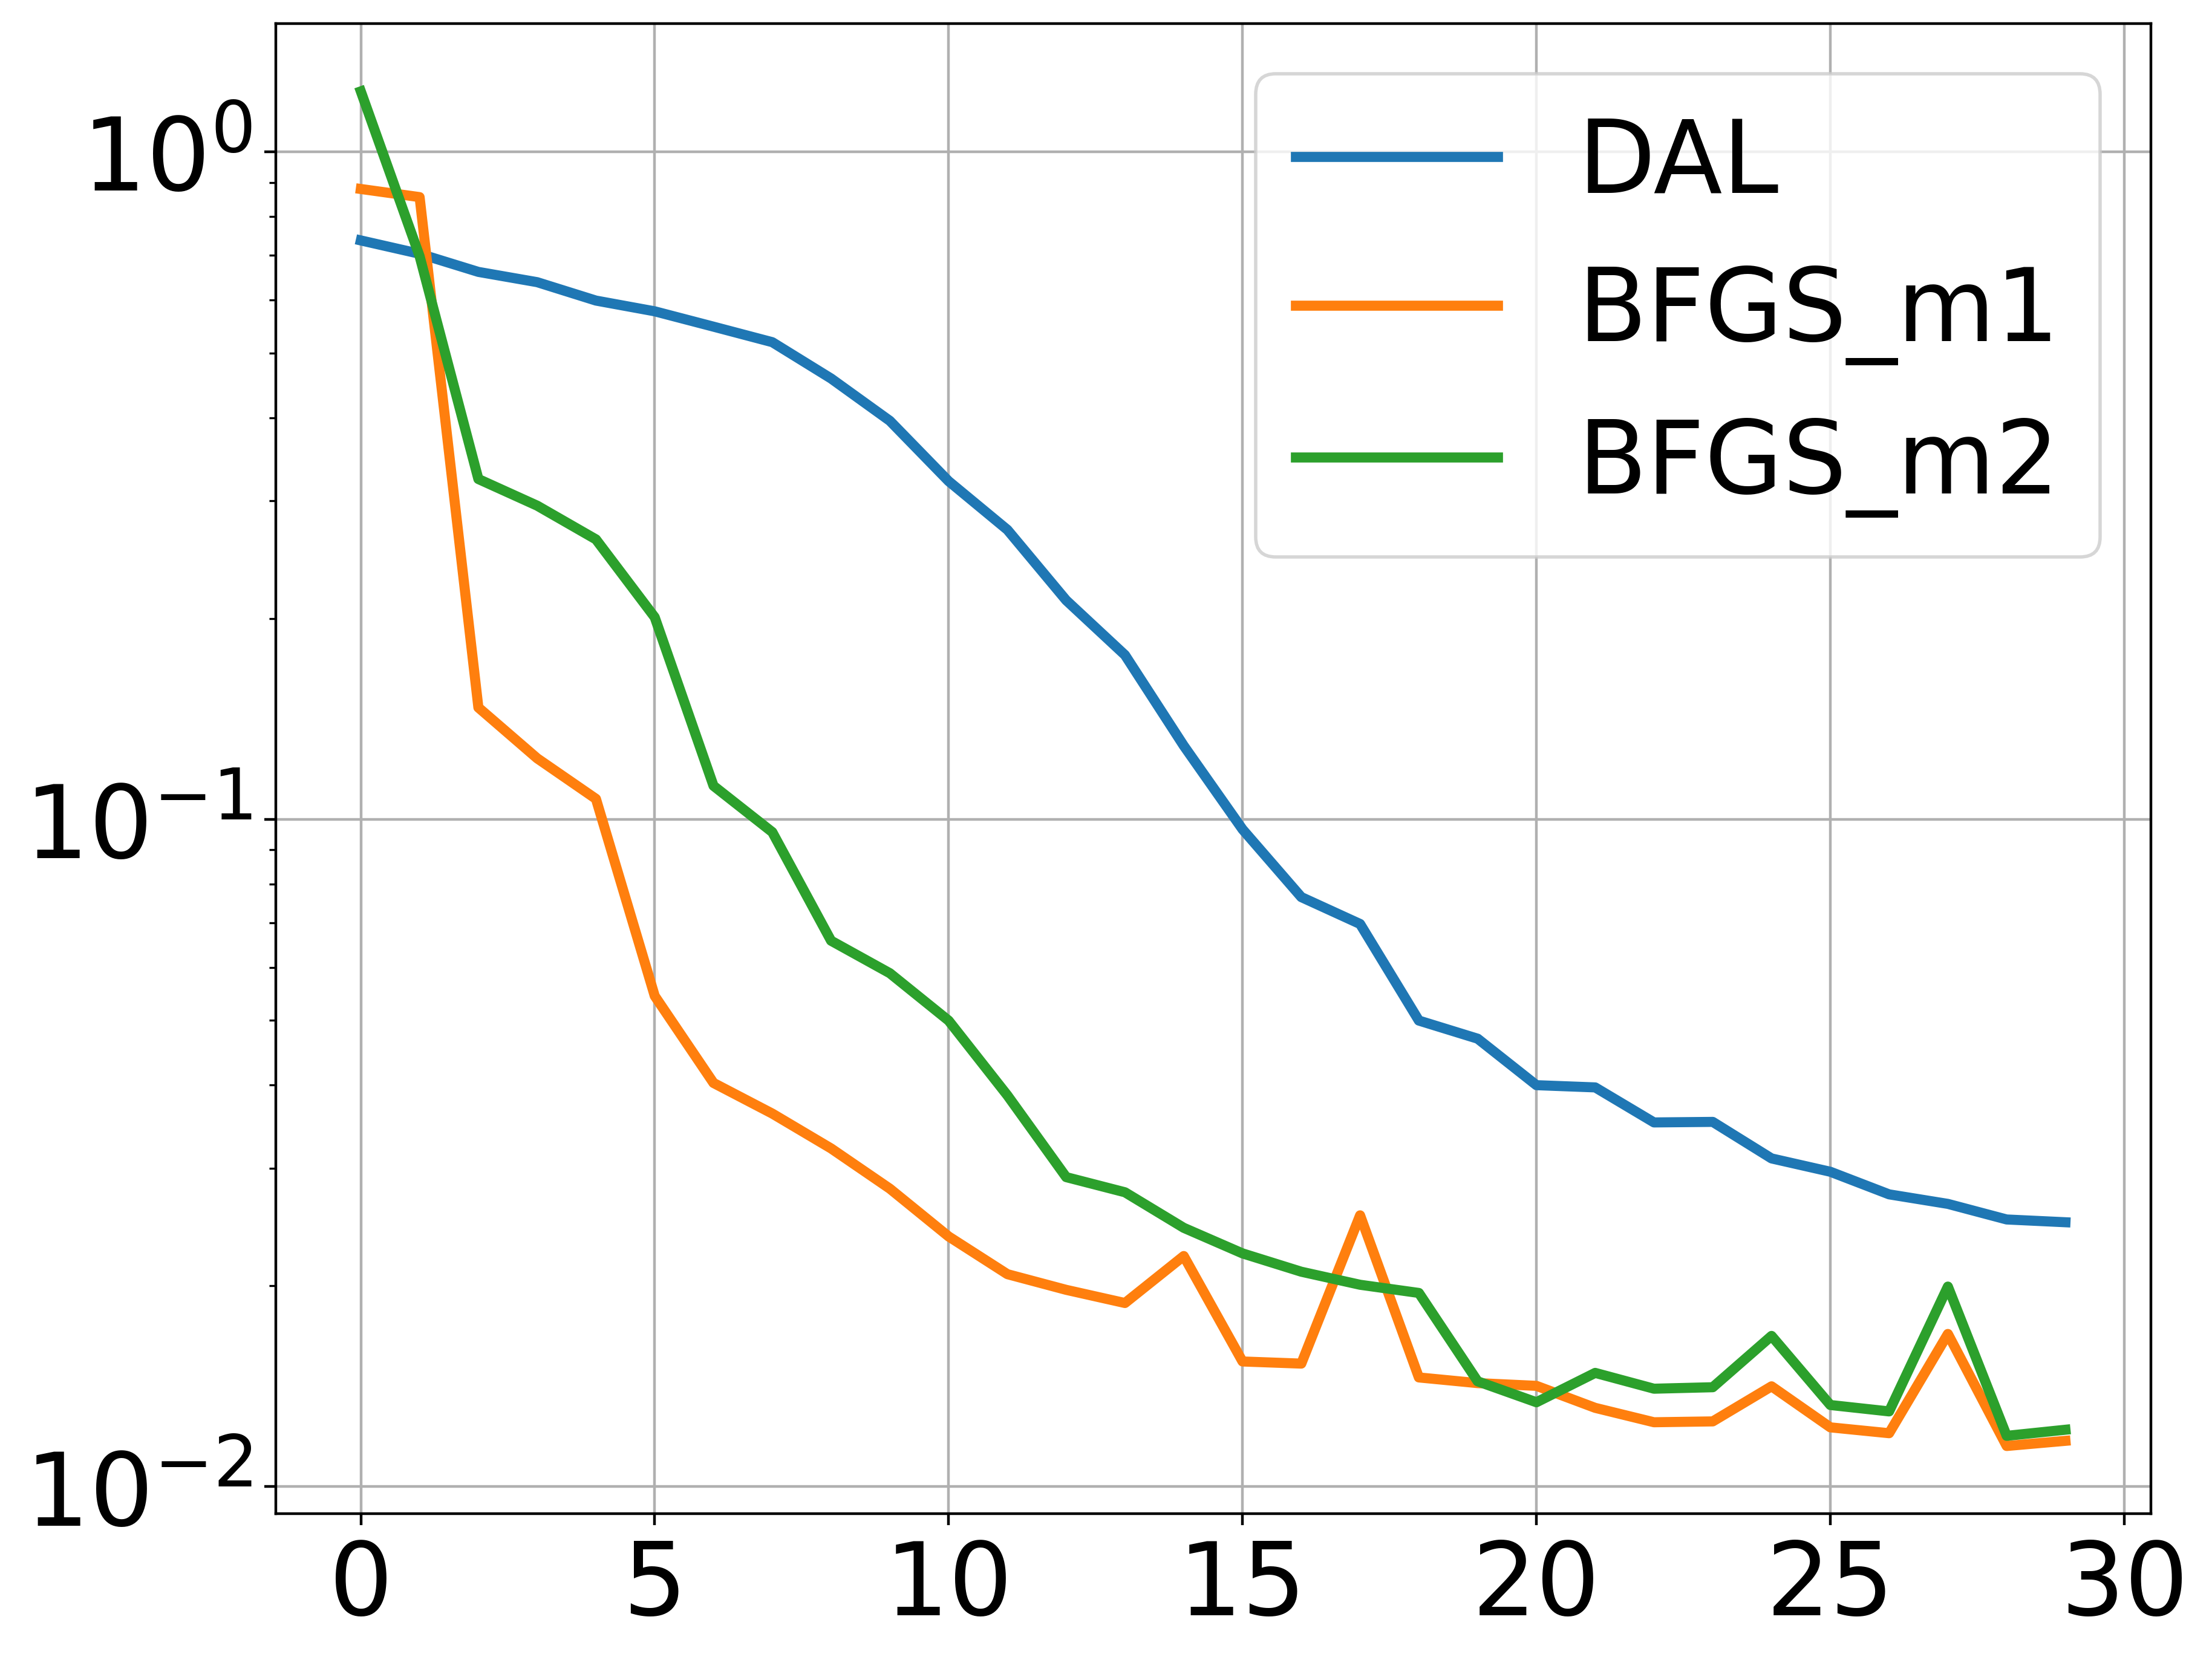
\includegraphics[width=0.3\textwidth]{figures/linear.png}
    &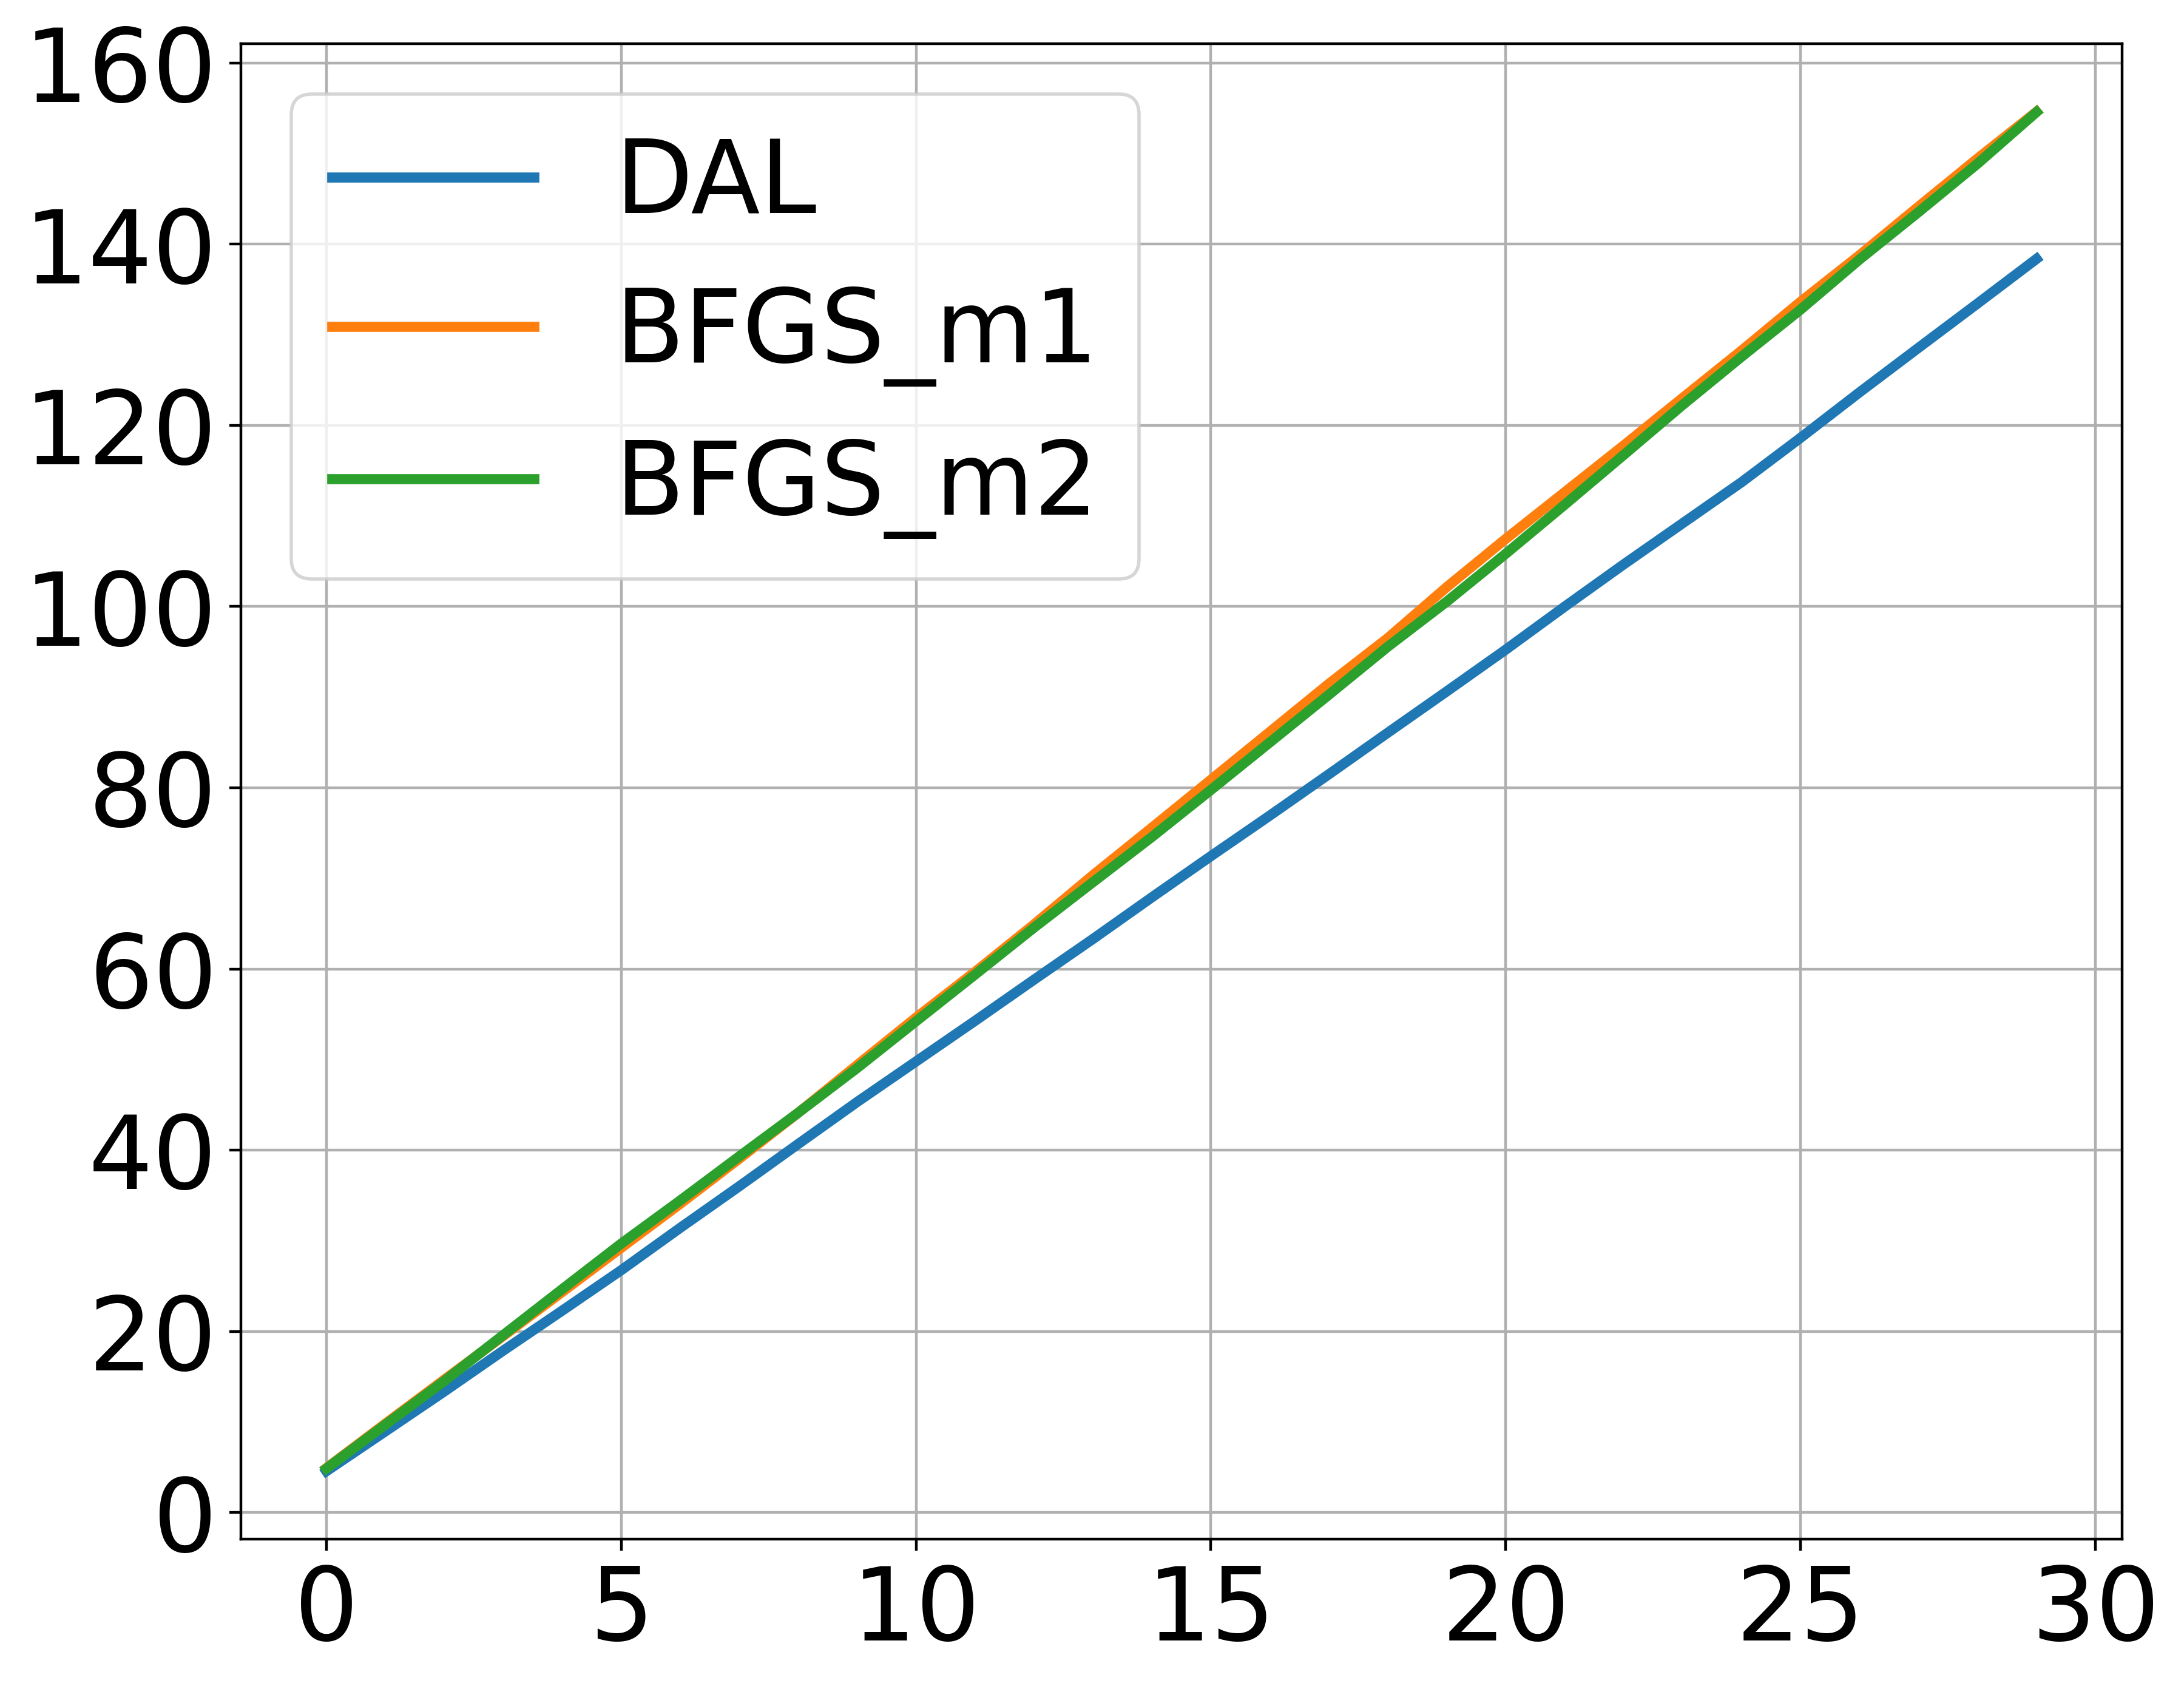
\includegraphics[width=0.3\textwidth]{figures/linear_time.png}
    &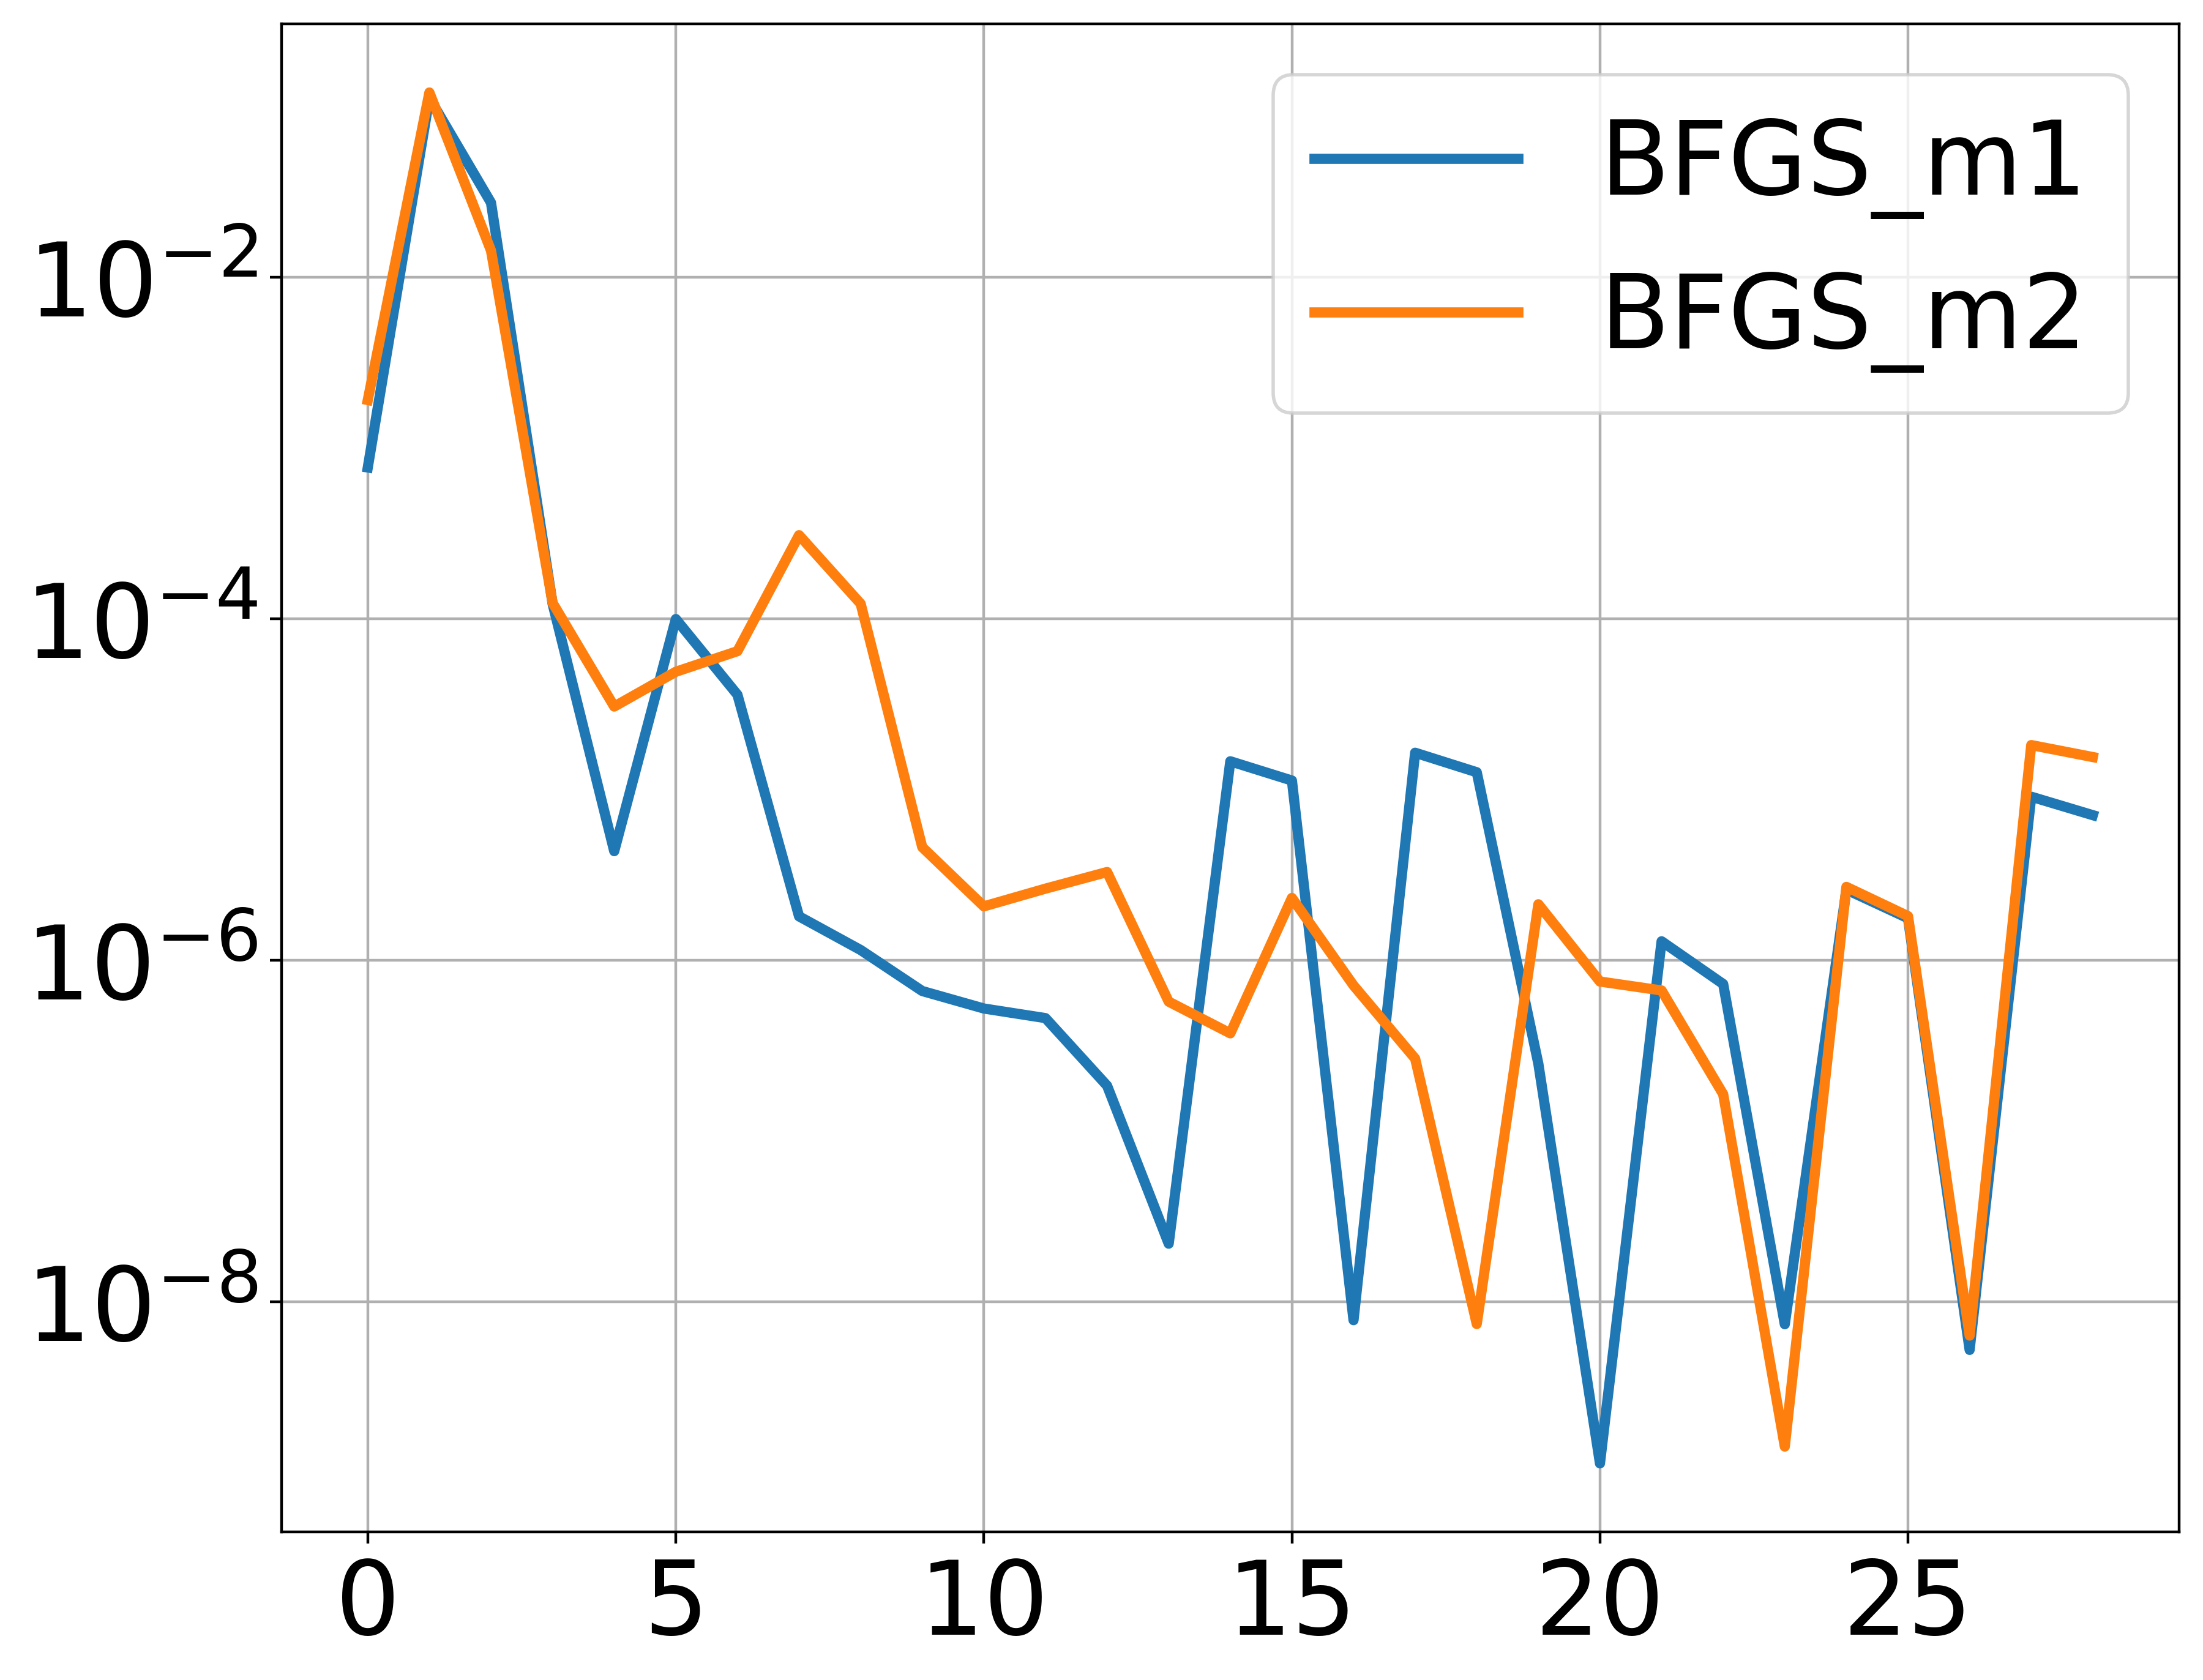
\includegraphics[width=0.3\textwidth]{figures/linear_curvcon.png} \\ 
    (a) Validation error & (b) Runtime & (c) Curvature
    \end{tabular}
    \caption{Linear annulus domain}
\label{fig:annulus_loss}
\end{figure}
Curvature condition for L-BFGS is satisfied, and the convergence rate is superior to first order method. Runtime of BFGS for each step is even slightly shorter, possibly due to a less line-search in the inner L-BFGS iteration. 

\paragraph*{Example 2} Linear Poisson on annulus domain, but the control is constrained.

Instead of using L-BFGS-B, we employ an additional projection after the gradient descent step. This will affect the convergence rate of BFGS, but offers flexibility to deal with various control constraints. 

\begin{figure}[hbt]
    \centering
    \begin{tabular}{cc}
    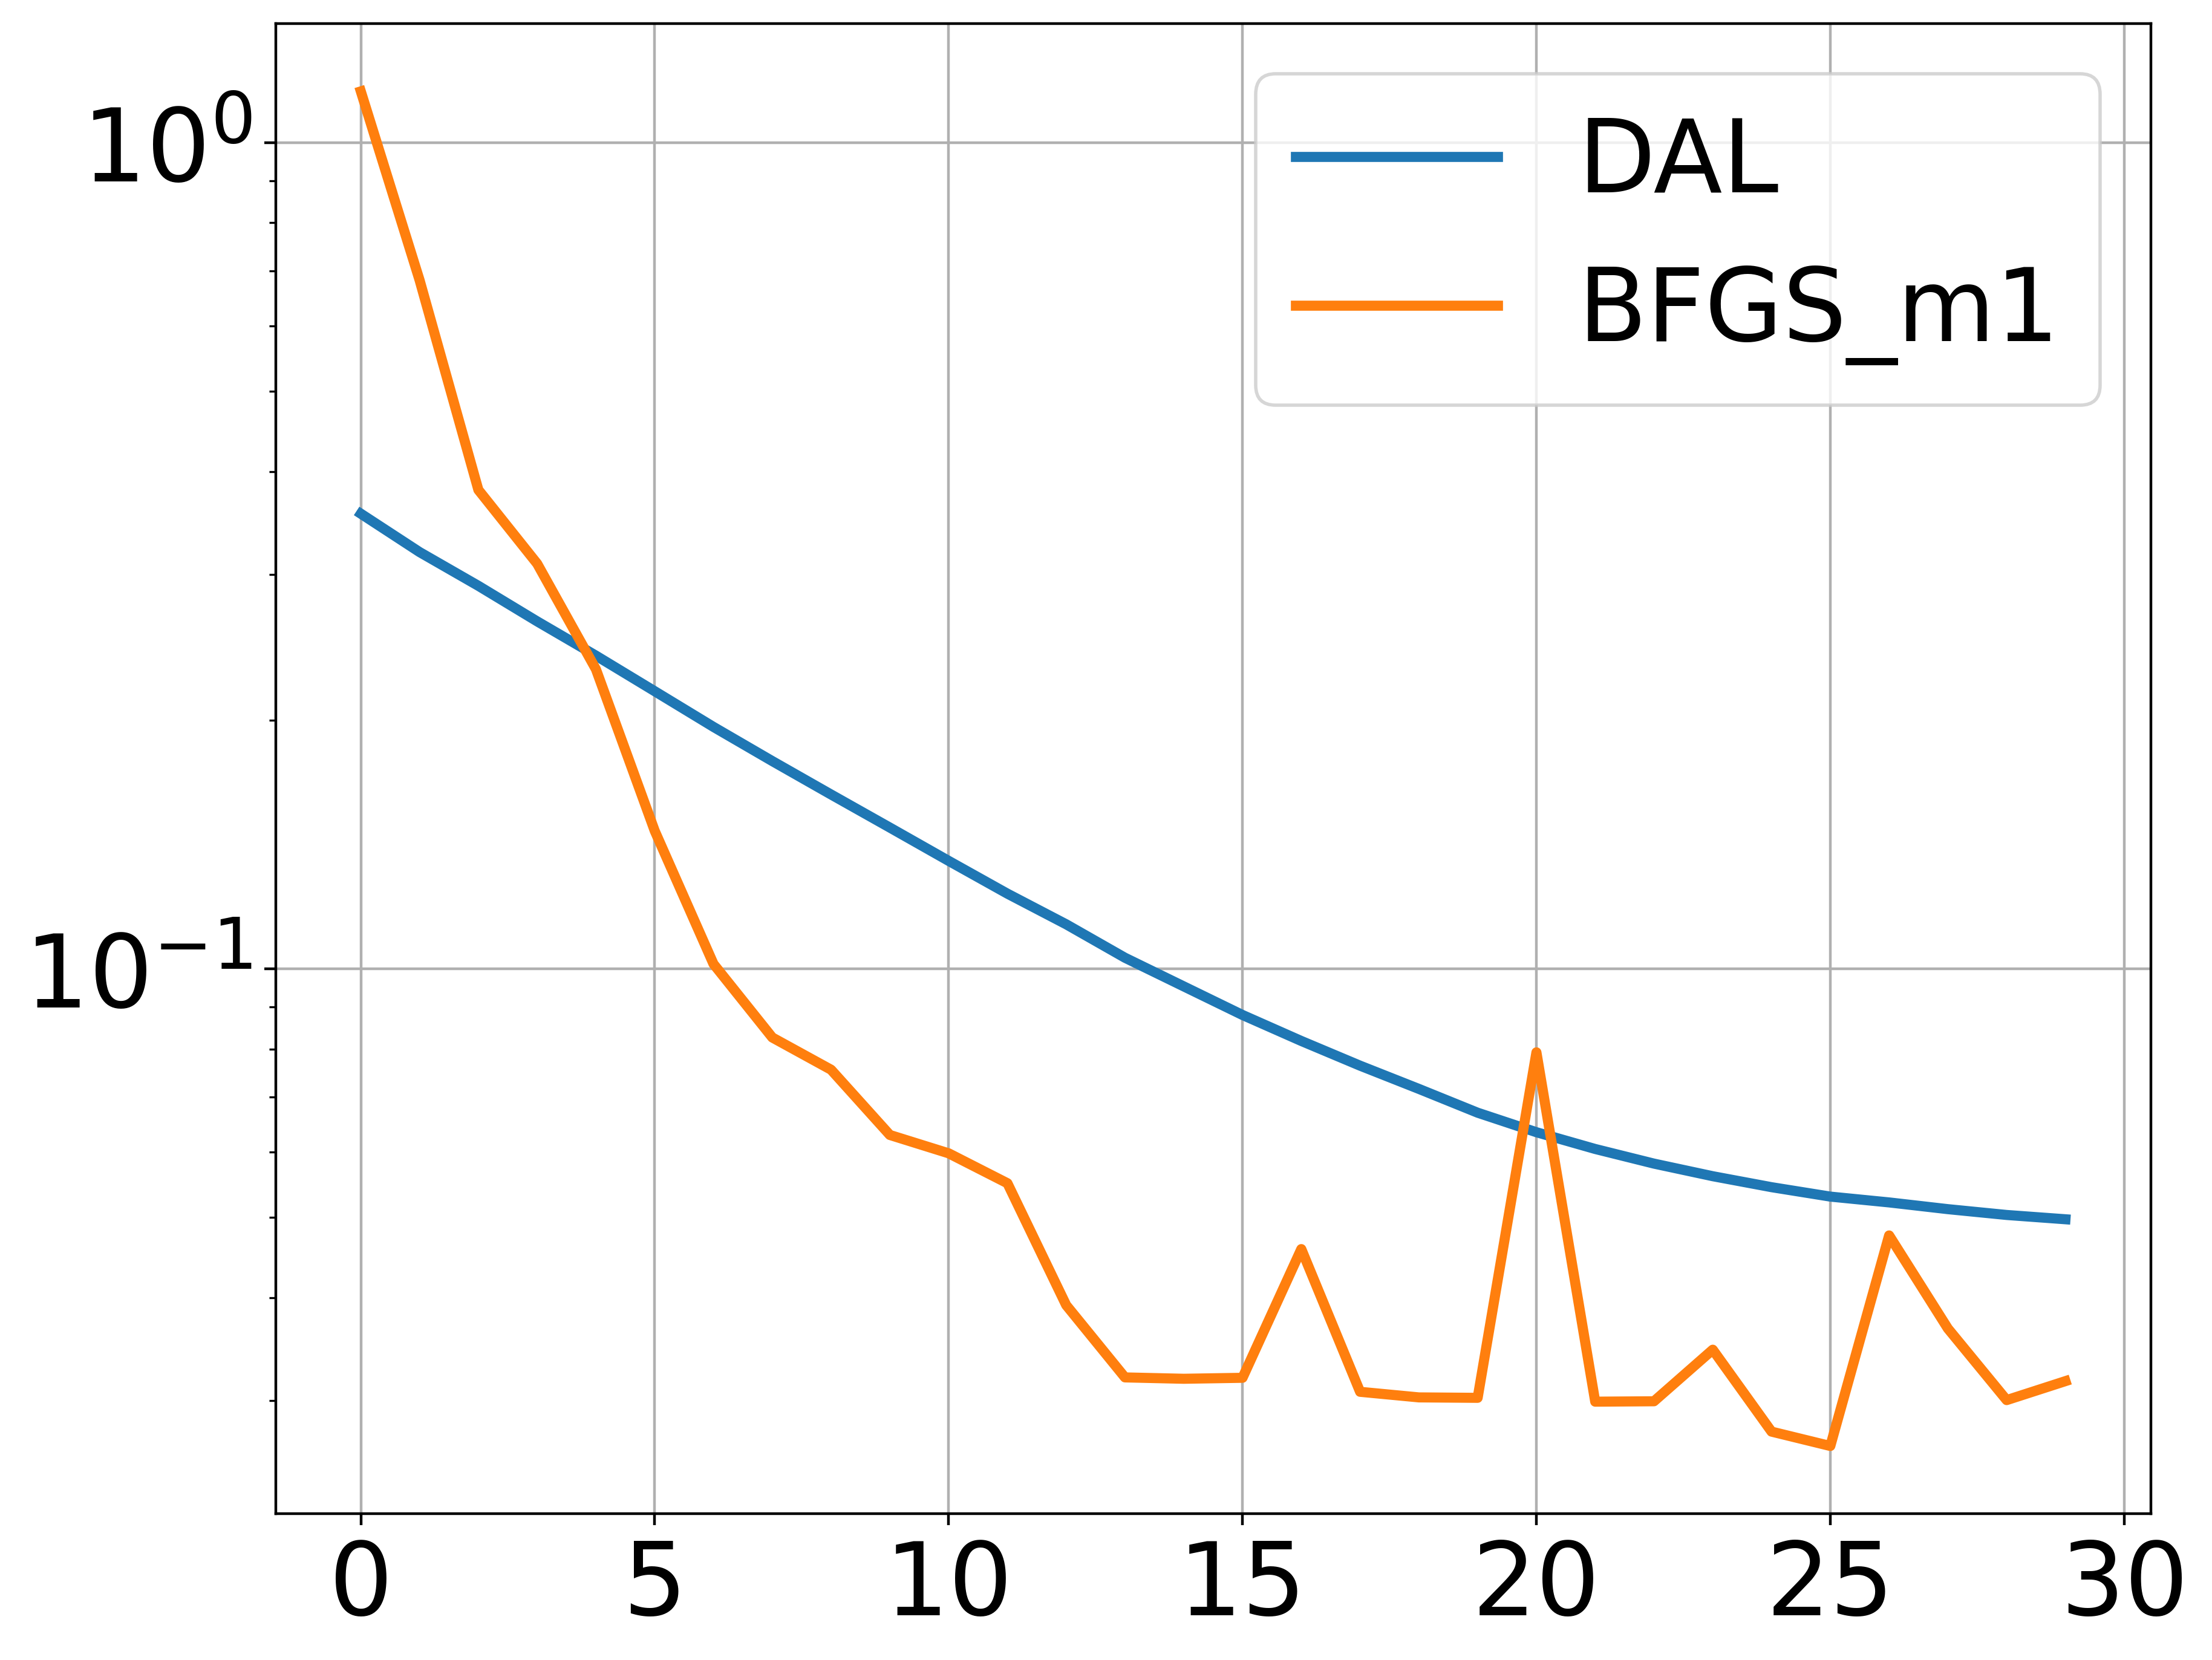
\includegraphics[width=0.45\textwidth]{figures/linear_ctd.png}
    &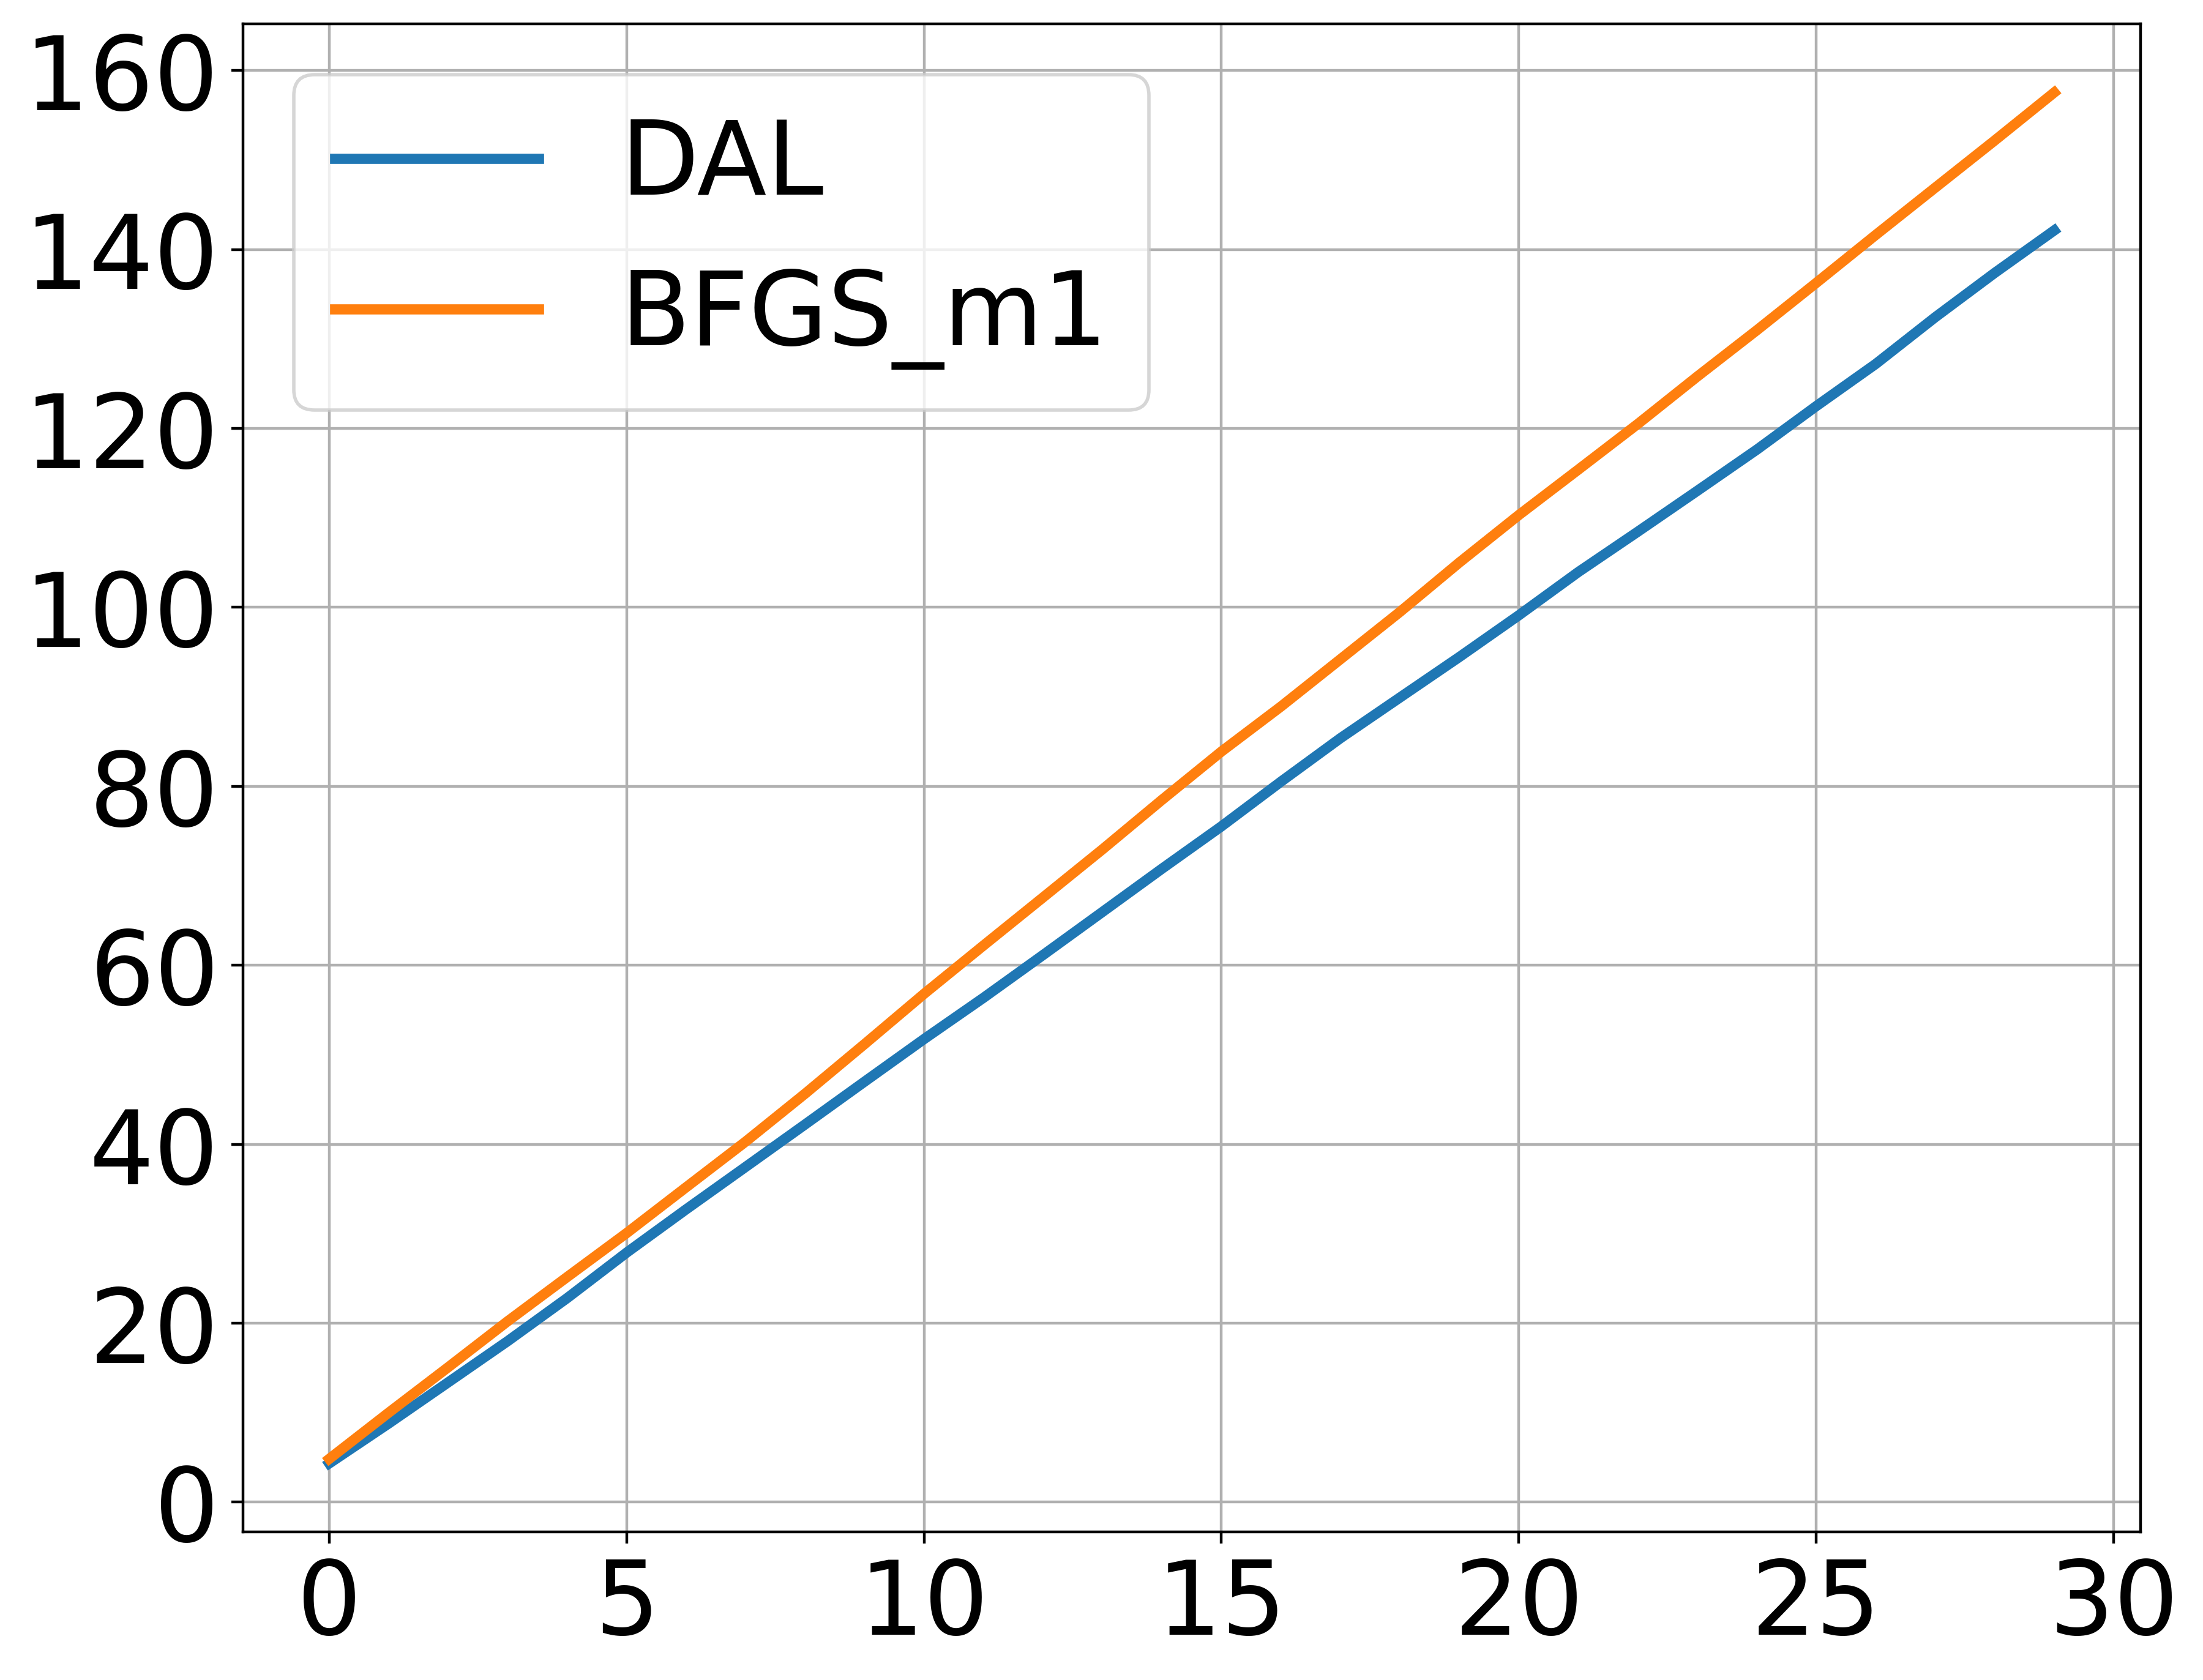
\includegraphics[width=0.45\textwidth]{figures/linear_ctd_time.png} \\ 
    (a) Validation error & (b) Runtime
    \end{tabular}
    \caption{Linear annulus domain with constraints}
\label{fig:annulus_loss_ctd}
\end{figure}

Still L-BFGS has slightly shorter runtime for each outer iteration, and the convergence rate is superior. 

\paragraph*{Example 3} Semilinear Poisson on square domain.

With a semilinear PDE as constraint, the optimization problem is no longer convex in terms of functions, hence first and second order methods may converge to different local minimals. 

\begin{figure}[hbt]
    \centering
    \begin{tabular}{cc}
    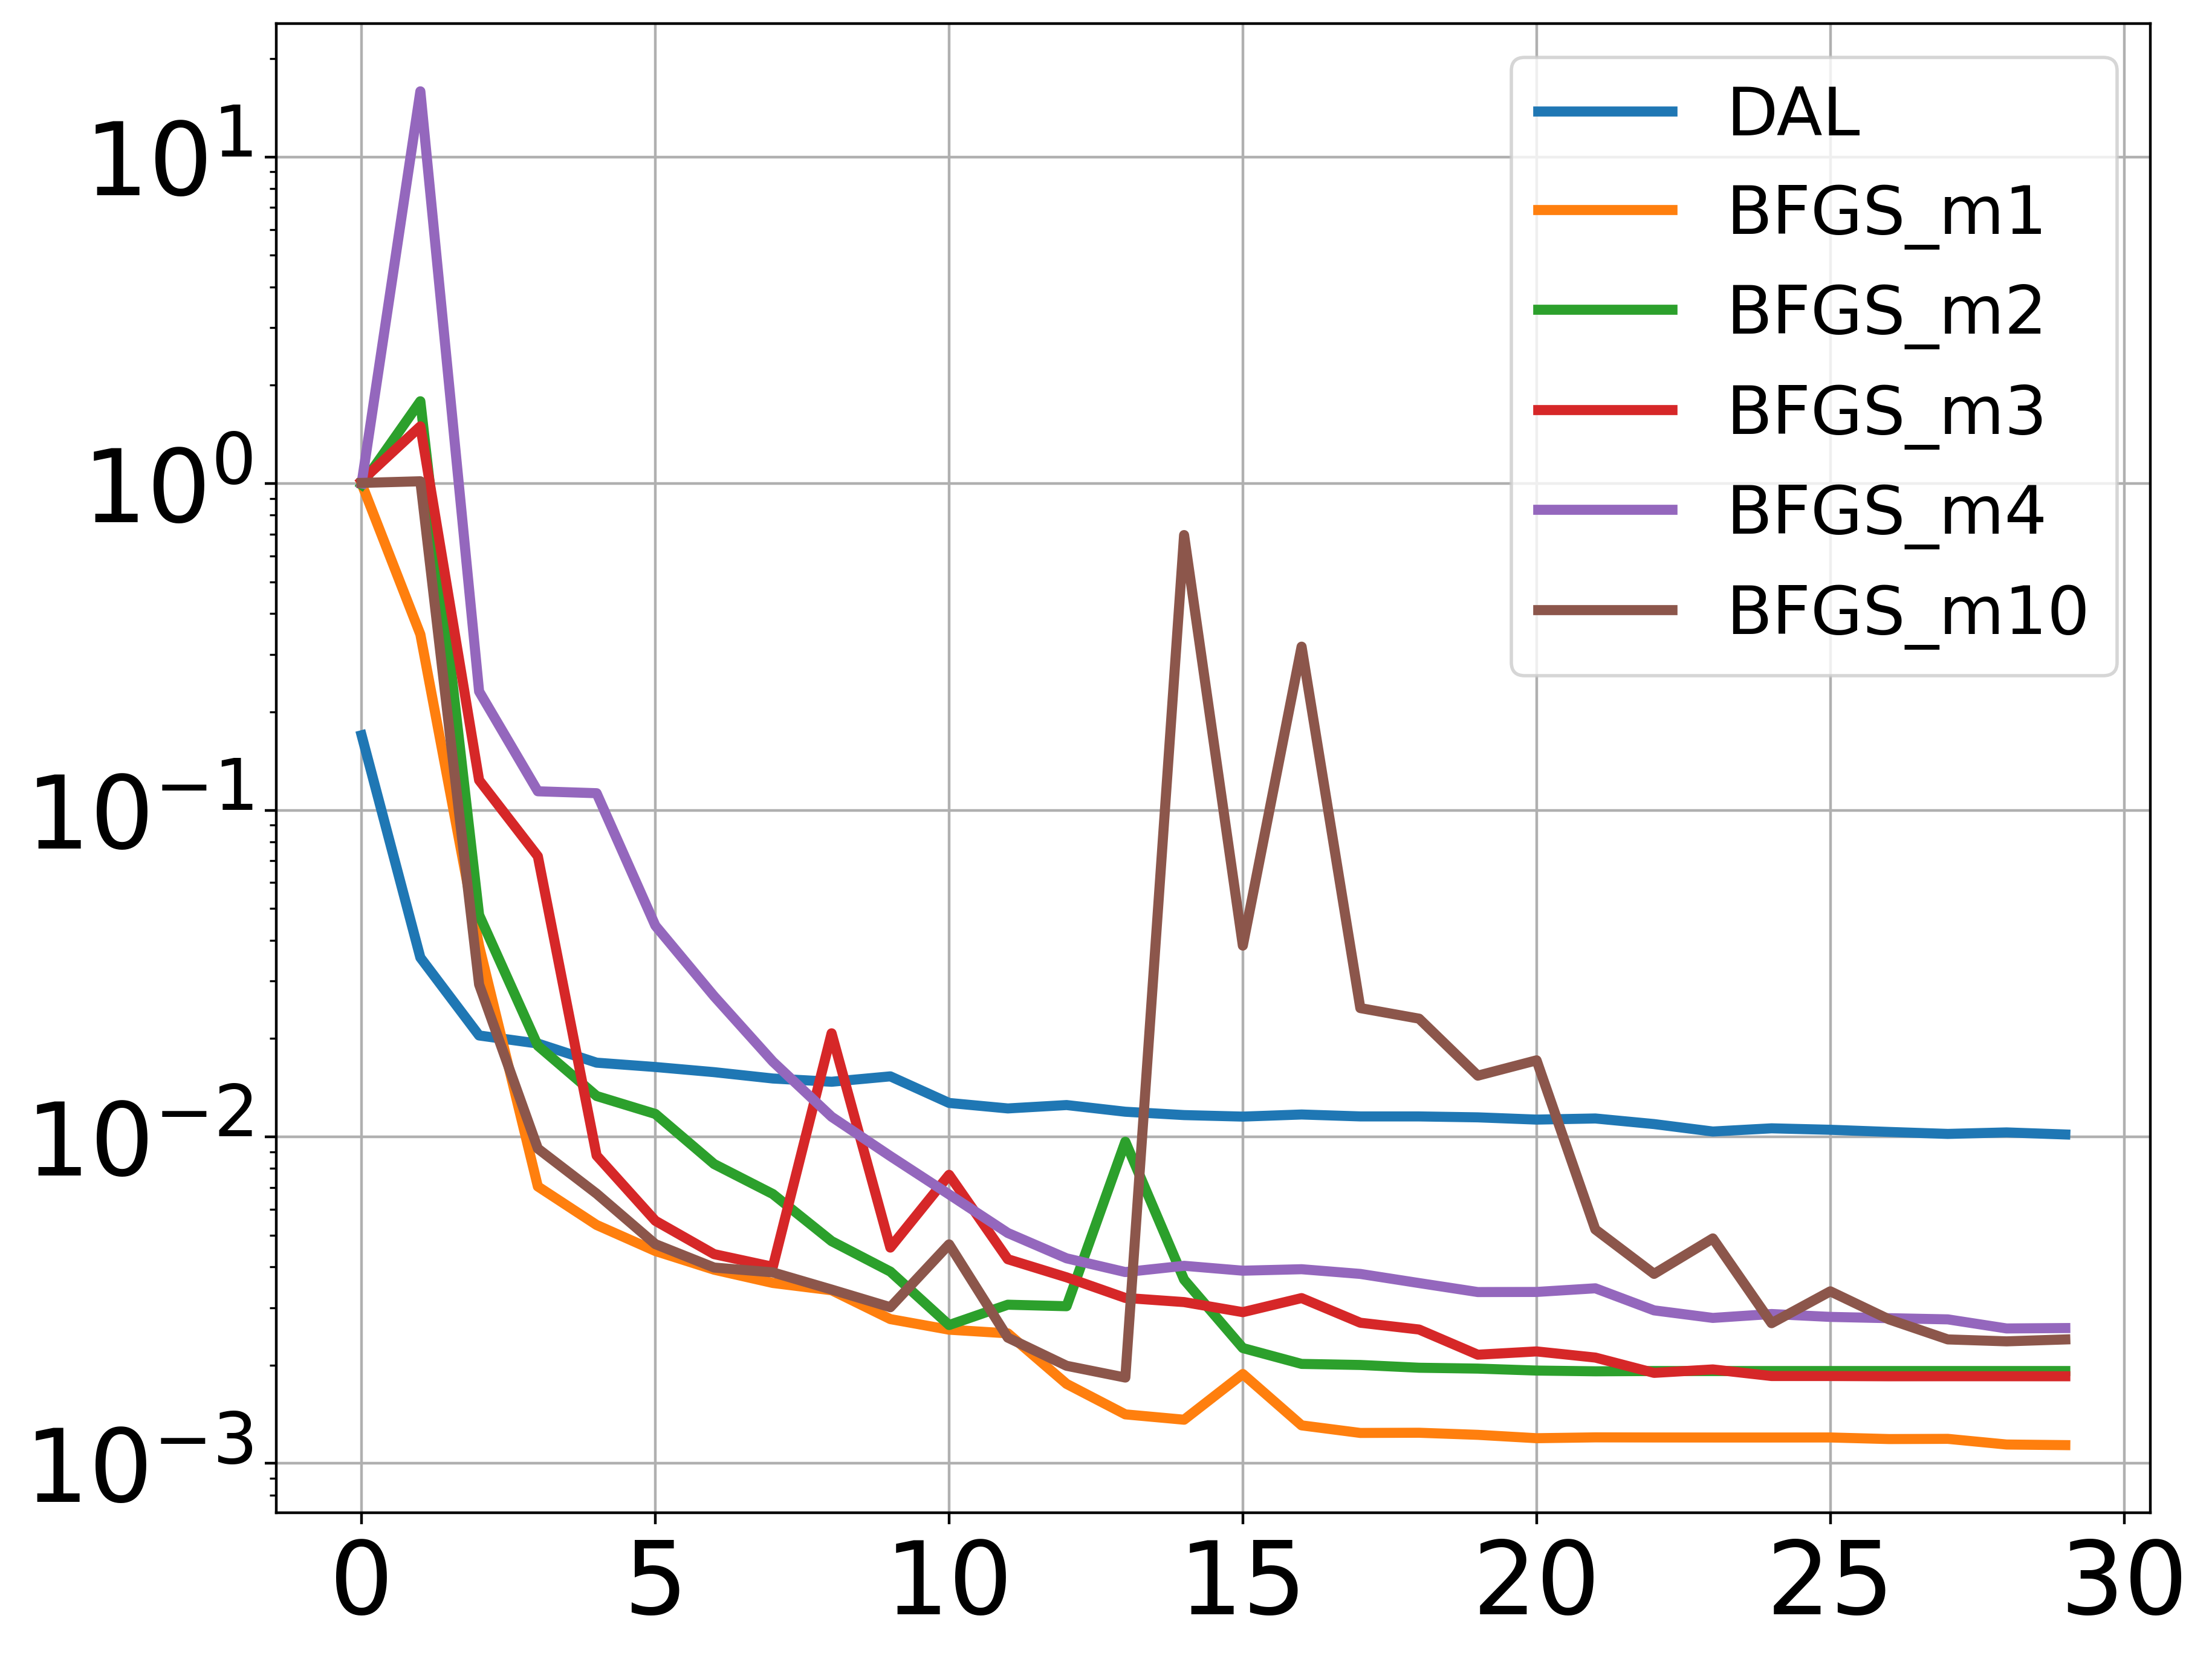
\includegraphics[width=0.45\textwidth]{figures/semilinear.png}
    &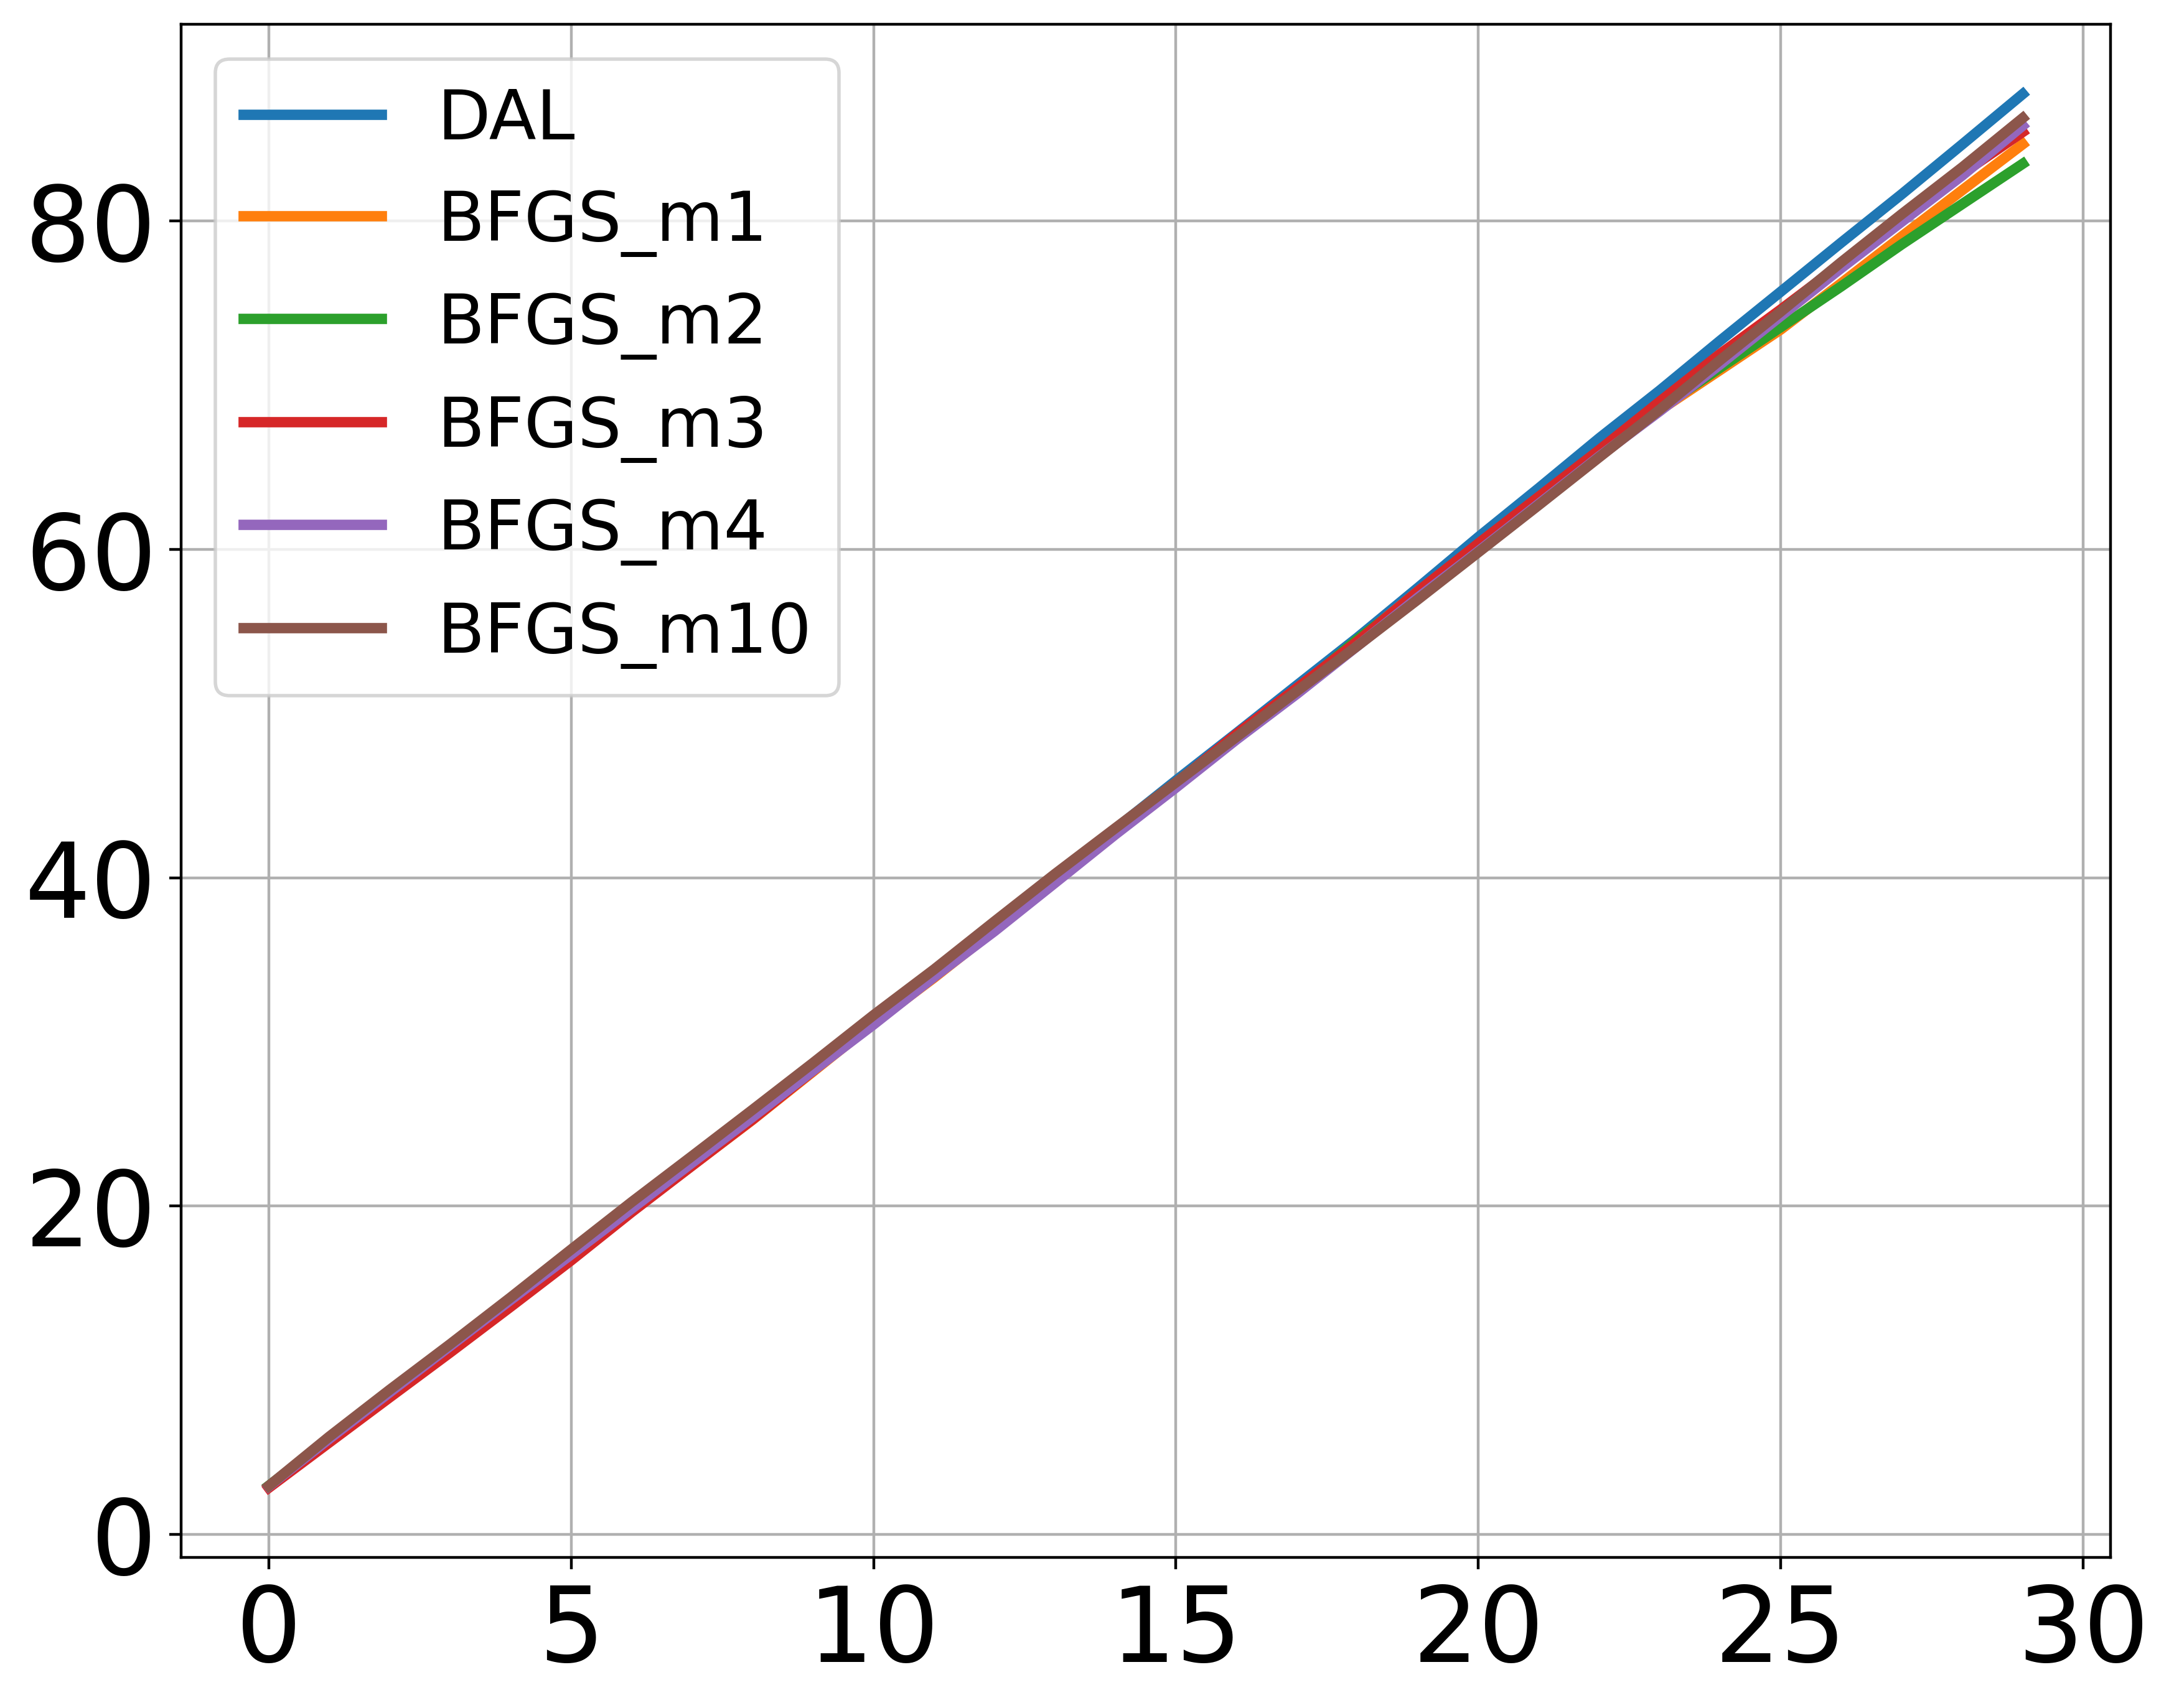
\includegraphics[width=0.45\textwidth]{figures/semilinear_time.png}\\ 
    (a) Validation error & (b) Runtime
    \end{tabular}
    \caption{Semilinear square domain}
\label{fig:semilinear}
\end{figure}

In this semilinear example, L-BFGS still has a good performance, but different initialization will lead to different optimizers.


\paragraph*{Example 4} NS equation on square domain with small Reynolds number.

NS equation is highly nonlinear and we test the difference of methods here.

\begin{figure}[hbt]
    \centering
    \begin{tabular}{cc}
    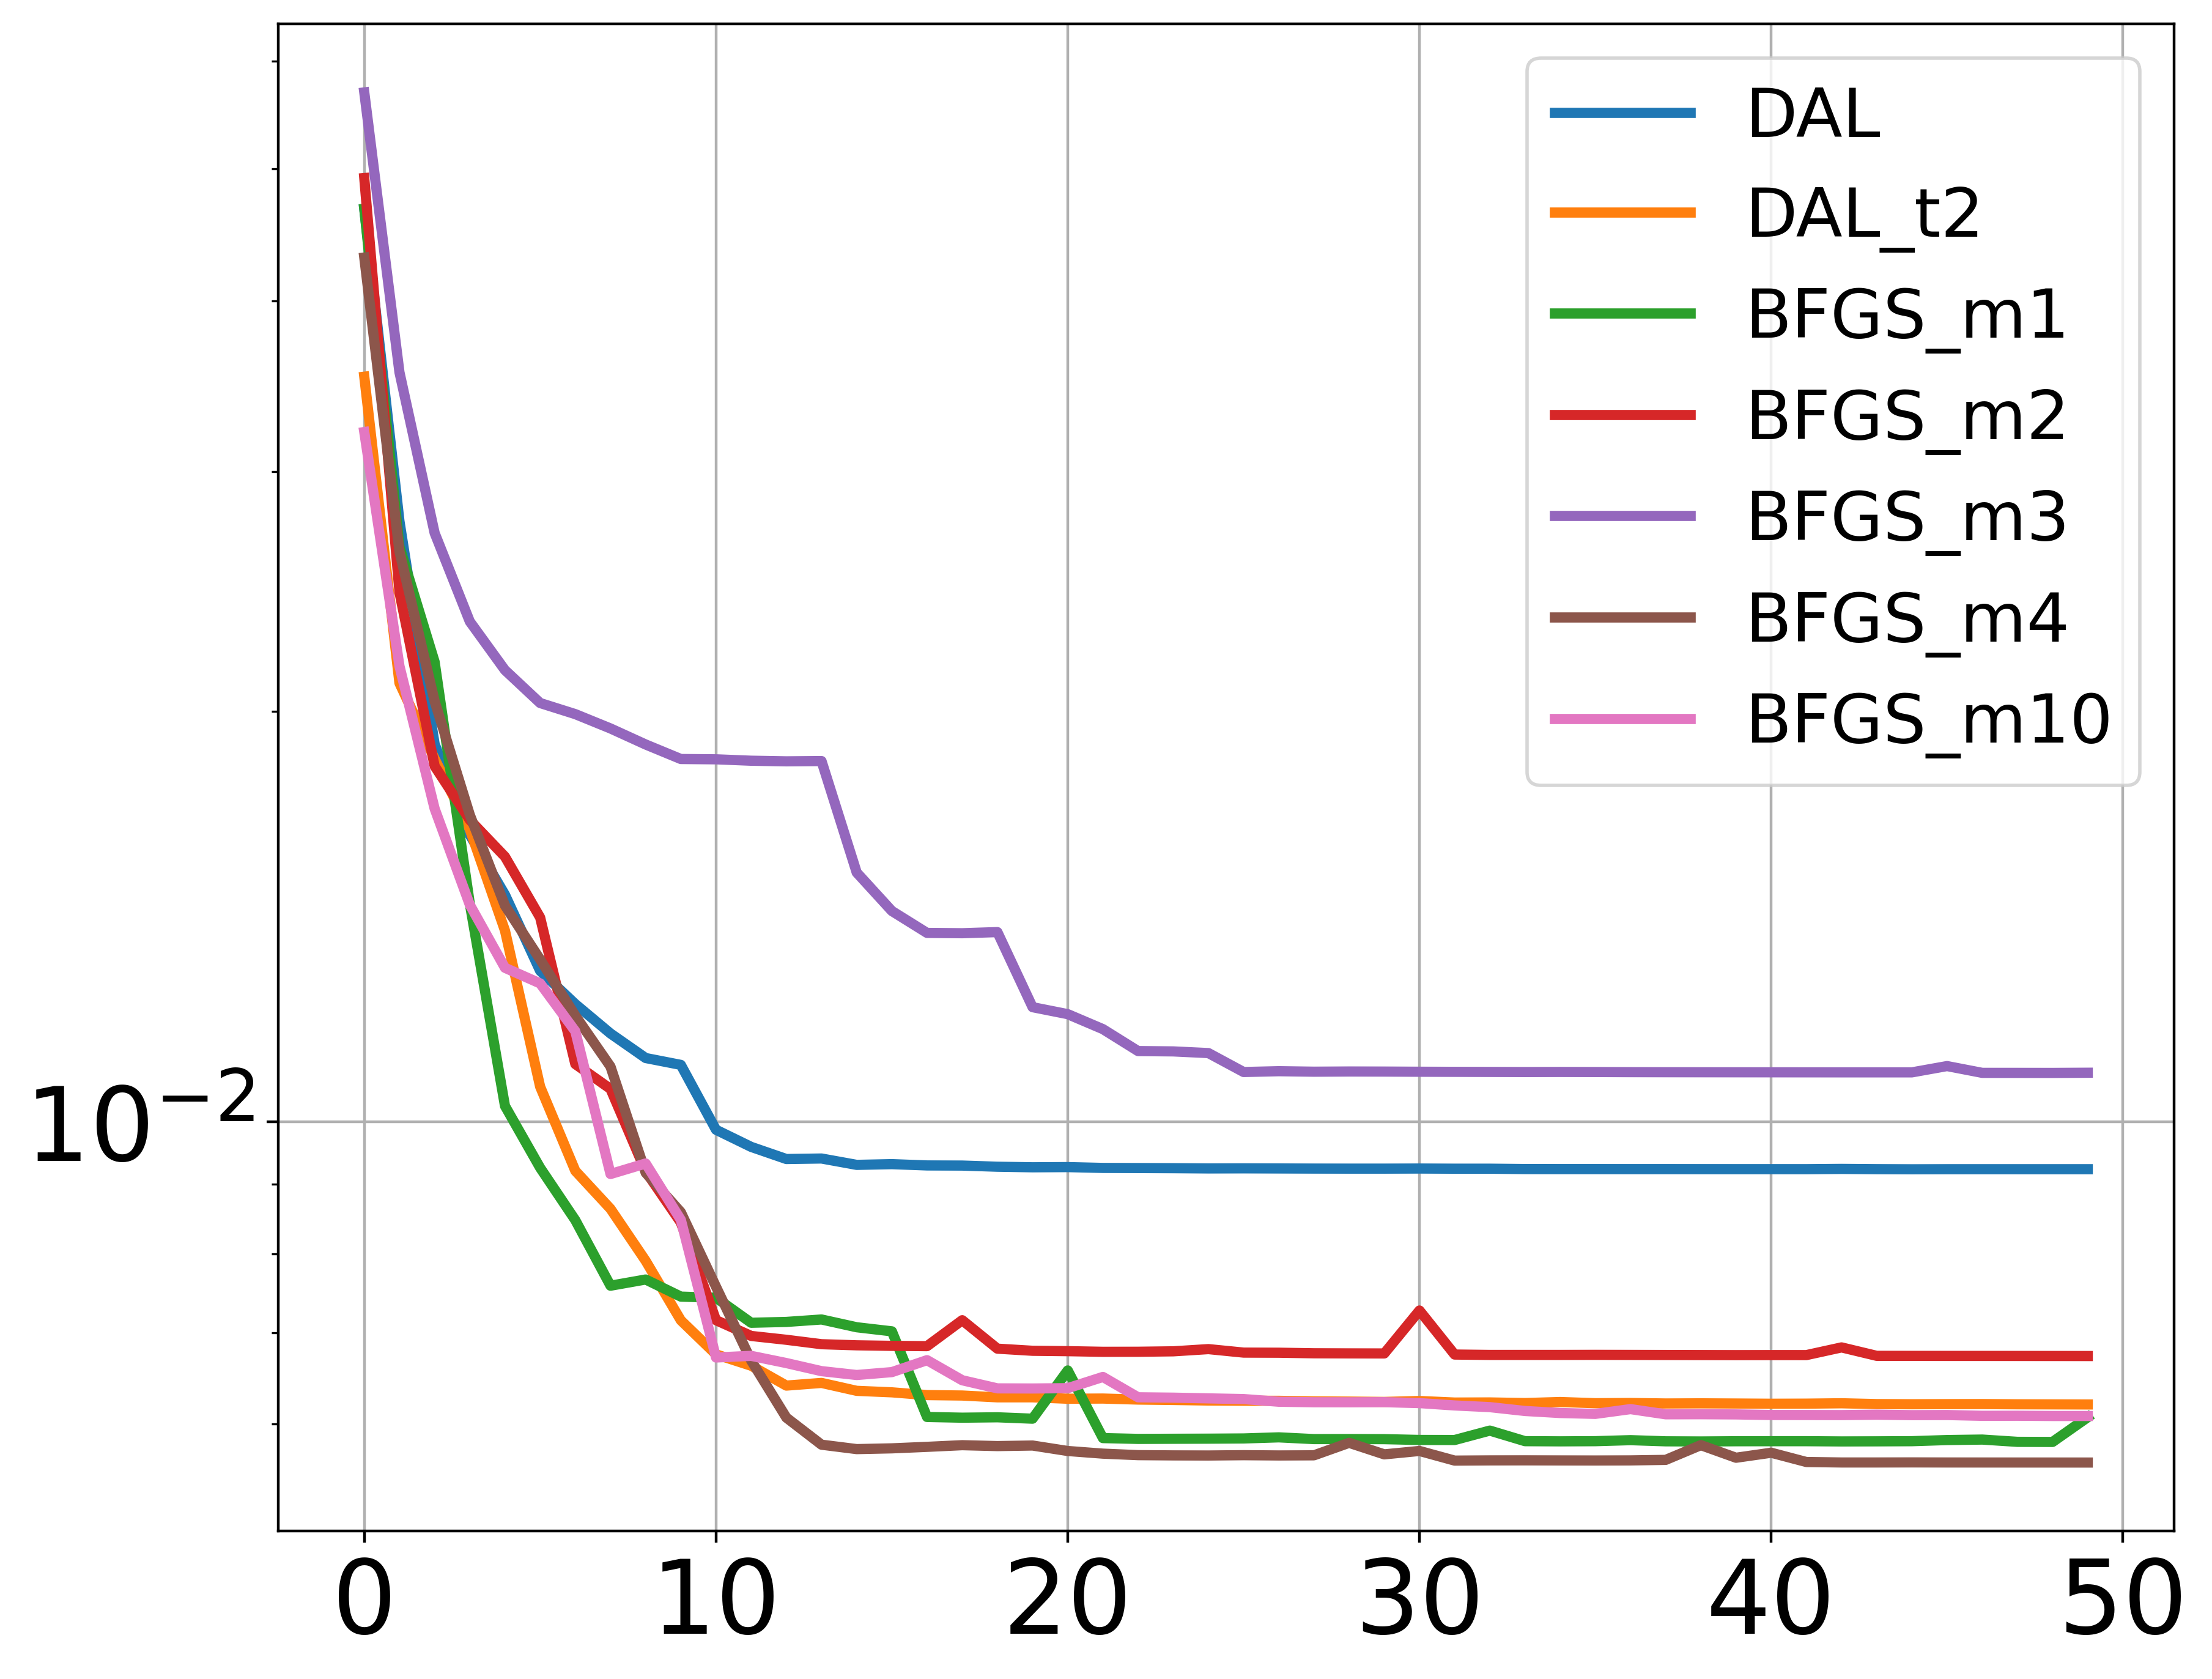
\includegraphics[width=0.45\textwidth]{figures/steadyNS.png}
    &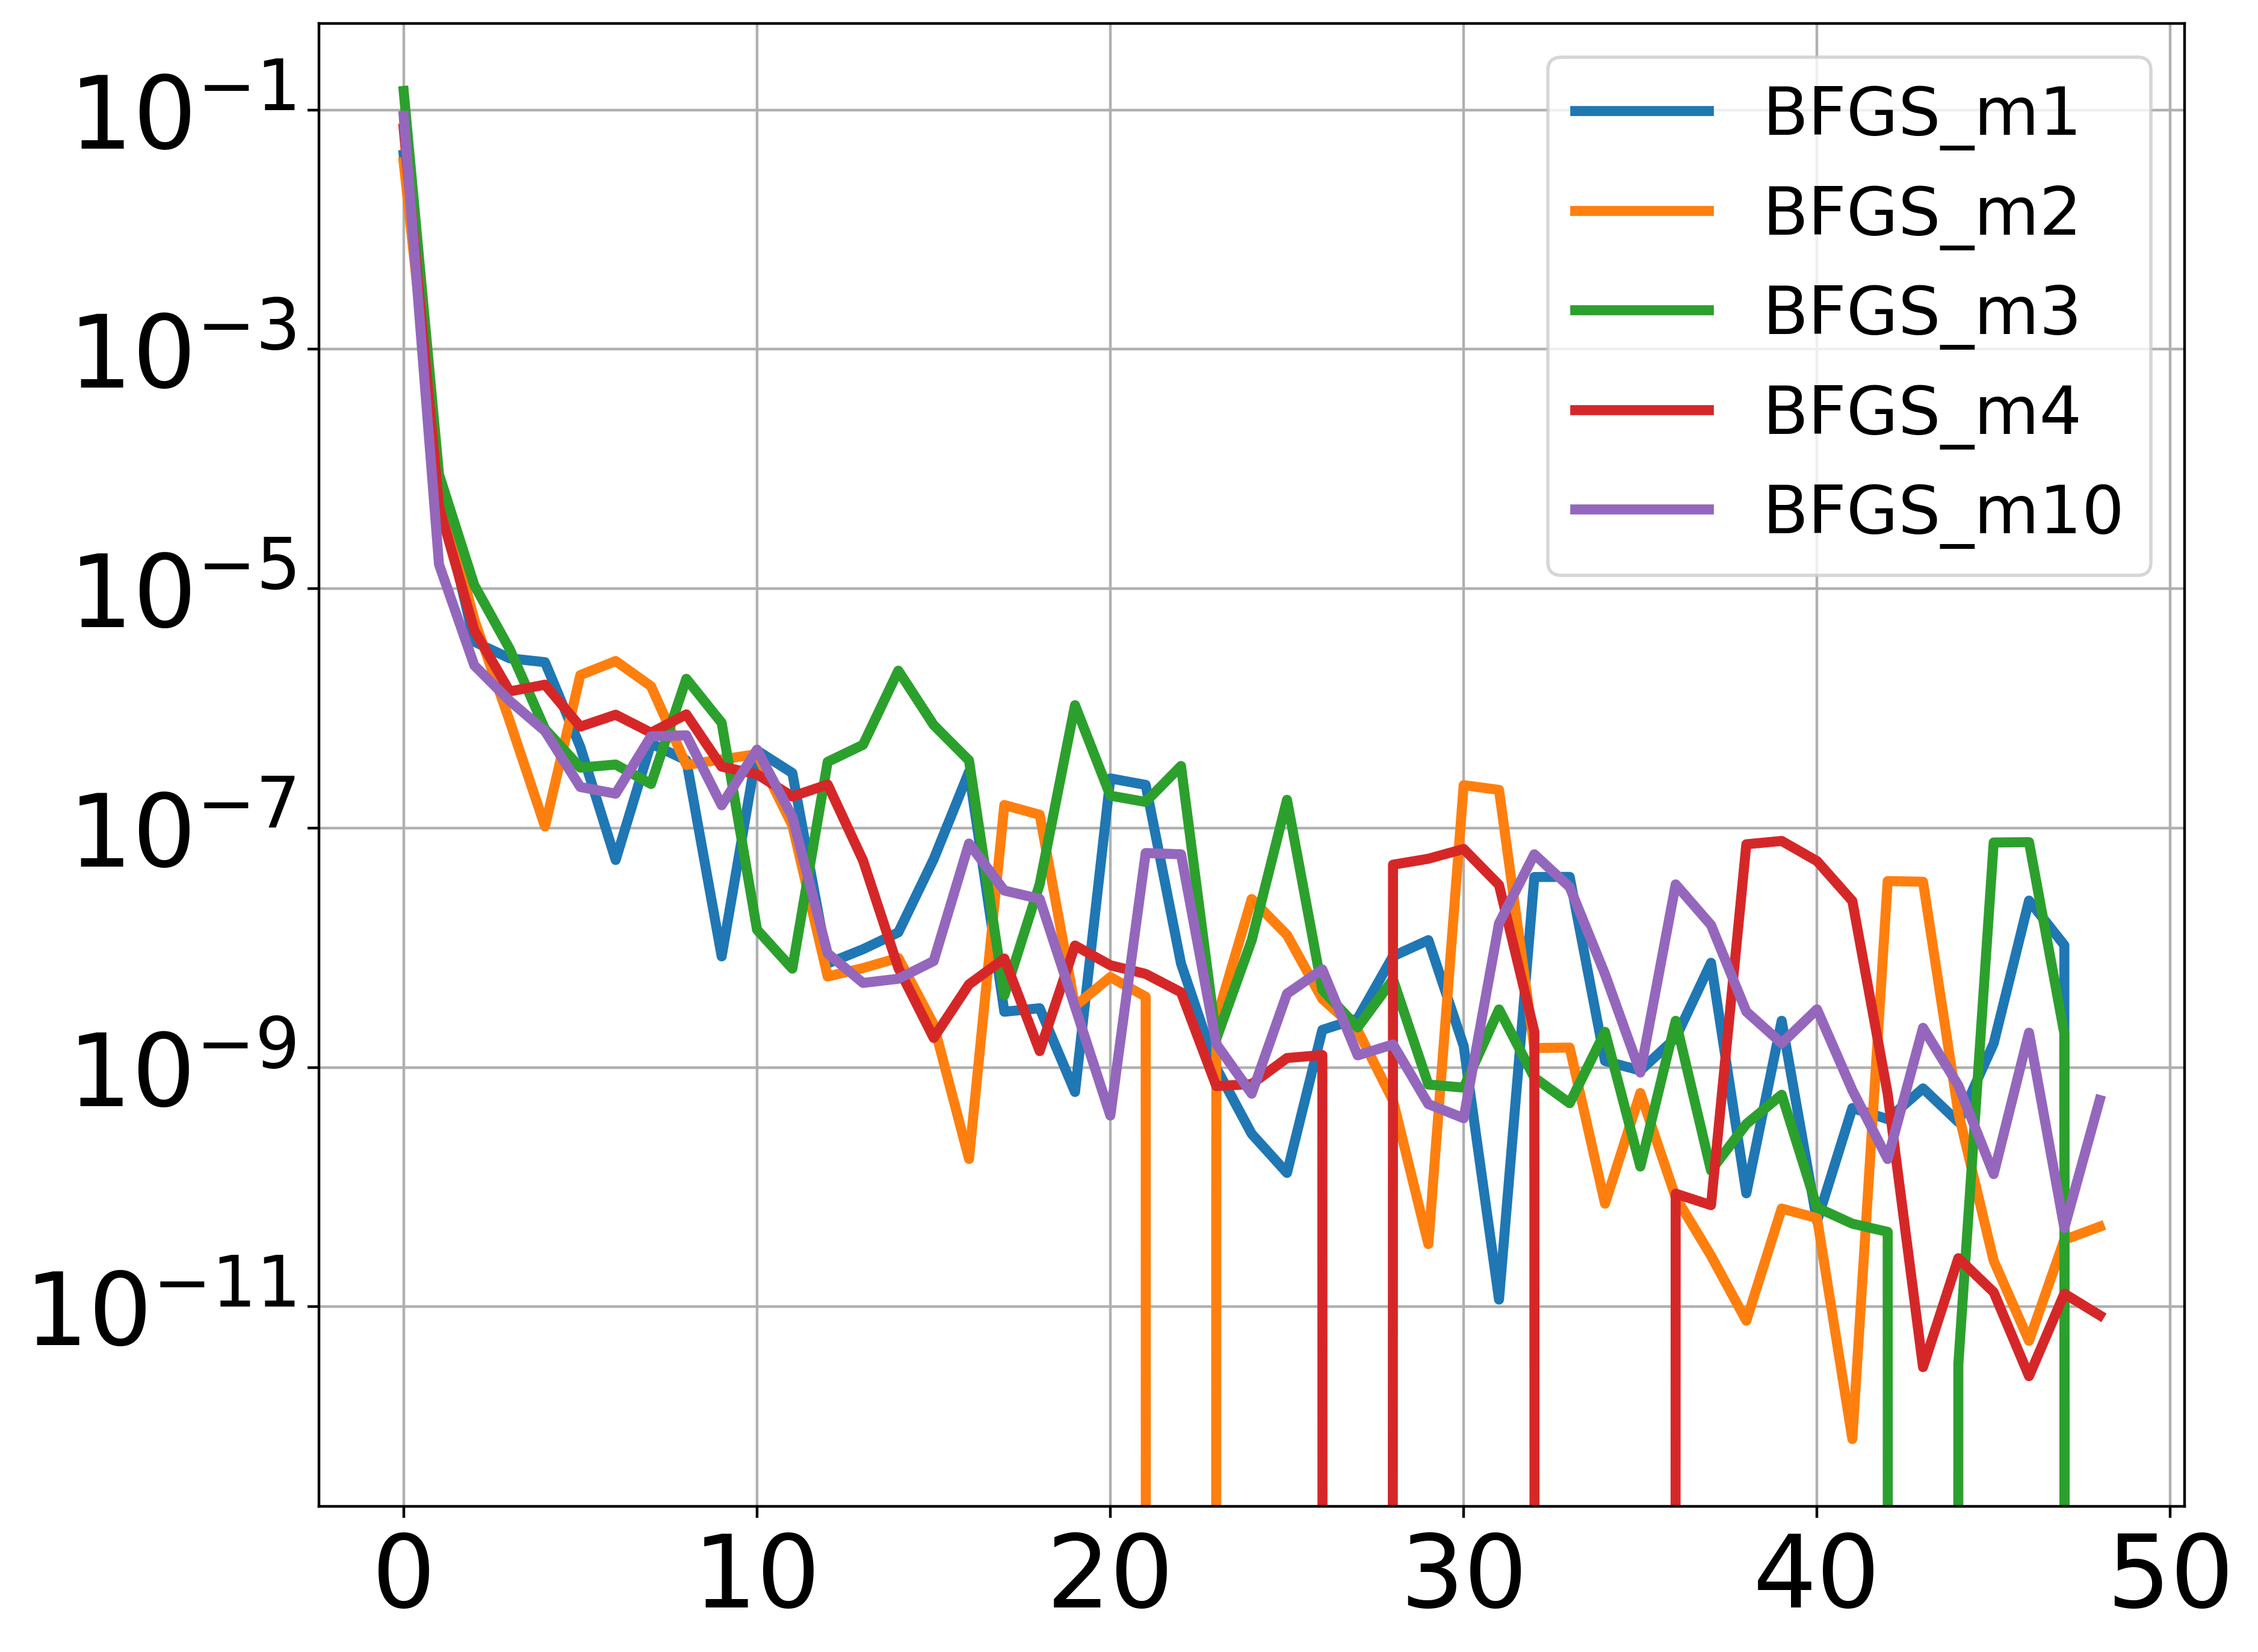
\includegraphics[width=0.45\textwidth]{figures/steady_NS_curvcon.png} \\ 
    (a) Validation error & (b) Curvature
    \end{tabular}
    \caption{NS equation}
\label{fig:NSeqn}
\end{figure}

It's found that during iteration, the curvature does not always hold positive. This is because the Hessian is not positive definite. The iteration of BFGS still converges, but does not show a superior convergence rate, and it is not guaranteed to converge to a local minimum that is better than first order methods. 


\end{document}

\end{document}